\chapter{Numerical relativity in short}\label{ch:nr_methods}

%In this thesis we perform numerical simulations of \ac{BNS} mergers. 
%The foundation of the \ac{NR} simulations is \ac{GR}, equations of which are 
%solved numerically. In this chapter we 
In the simulations the \ac{EFE} describing the spacetime dynamics, are formulated in a 
way more suitable for numerical applications. We discuss this formulations in 
Sec.~\ref{sec:nr_methods:nr}, where we summarize the equations for \ac{NR}.
The basis of \ac{EFE} and \ac{GR} is not covered here for the sake of brevity. For that we 
refer to \citet{Arnowitt:1962hi,Landau:1982dva,Wald:1984,Misner:1973,Baumgarte:2002jm}.


\section{Numerical implementation of General Relativity}\label{sec:nr_methods:nr}

%%%% === Additional Intro
%The \ac{EFE} is the foundation of modern cosmology, the physics of \acp{NS} and \acp{BH},
%the emission of gravitational radiation, and numerous other cosmic phenomena, 
%where strong gravity effects are present. The Einstein theory of \ac{GR} has 
%passed numerous tests in the weak-field regime \citep{Asmodelle:2017sxn} and in a 
%strong field regime when the gravitaional radiation from the merger of two \acp{BH} was 
%detected for the first time \citep{Abbott:2016blz}.

\ac{EFE} in a covariant form, neglecting the cosmological constant, read
%
\begin{equation}
    G_{\mu\nu} = R_{\mu\nu} - \frac{1}{2} R g_{\mu\nu} = 8\pi T_{\mu\nu}
    \label{eq:theory:EFE}
\end{equation}
%
%(As an exercise we provide a short derivation of the 
%\ac{EFE} from the variation of Hilbert action in Appendix~\ref{app:efe})
%
where $R_{\mu\nu}$ is the Ricci curvature tensor with its trace 
$R^{\mu}_{\nu} = R$, $g_{\mu\nu}$ is the metric tensor and 
$T_{\mu\nu}$ is the stress-energy tensor.

For numerical applications it is desirable to represent Eq.~\eqref{eq:theory:EFE} 
as an \ac{IVP}.
%, where once the initial data is specified at the time zero, 
%the evolution can be computed. 
This is highly non-trivial task. One of the commonly used methods is to perform 
\textit{$3+1$ decomposition}, where the $4$D 
manifold is represented as foliation of $3$D spacelike hypersurfaces 
\citep{Alcubierre:2008,Baumgarte:2010,Gourgoulhon:2007ue,Rezzolla:2013}.


\subsection{3+1-Decomposition}

\begin{figure}[t]
    \centering 
    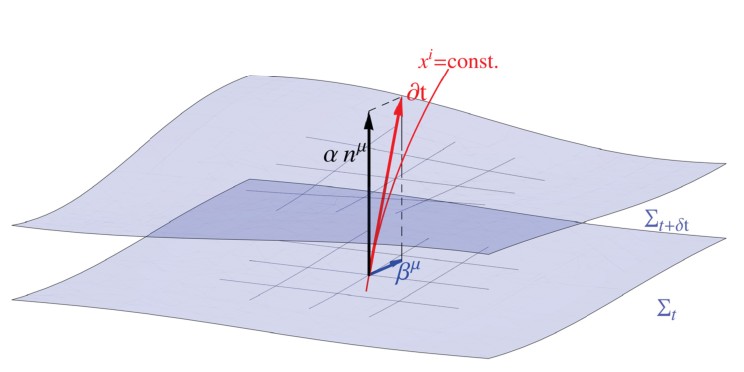
\includegraphics[width=0.49\textwidth]{tim_3p1_plot.pdf}
    \caption{
        Visual representation of the $4$D manifold $\mathcal{M}$ by $3$D hypersurfaces 
        $\Sigma_t$. The lapse function $\alpha$ and shift vector $\beta^{\mu}$ describe the 
        coordinate change between hypersurfaces.
        Adopted from \citet{Dietrich:2016phd}.
    }
    \label{fig:theory:3p1}
\end{figure}

Eq.~\eqref{eq:theory:EFE} represent a set of $10$ non-linear \acp{PDE} 
that can be defined on a whole metric $\mathcal{M}$ or a domain $\Omega\subset\mathcal{M}$ 
%where in the latter case, the boundary conditions on 
with the boundary, $\partial\Omega$% are required. 
%
The initial data is defined on a null hyersurface $\Sigma\subset\mathcal{M}$. 
The subsequent evolution requires that the foliation 
$\mathcal{M}=\Sigma\times\mathbb{R}$, depicted in Fig.~\ref{fig:theory:3p1}, 
is allowed, or in other words, that the spacetime is strongly hyperbolic. 
%
%This foliation can be understood as splitting the spacetime into a set of 
%spacelike hypersurfaces $\Sigma_t$ as depicted in Fig.~\ref{fig:theory:3p1}. 


%%%% ==== Basicas of Foliations, Lapse, Shift, Norm
Let $t$ be the global smooth functions such that 
$\Sigma_{\tau} = \{x^{\alpha}\in\mathcal{M}: t(x^{\alpha})=\tau\}$ 
and let $\vec{t}$ be a vector such that $\langle\nabla t, \vec{t}\rangle = 1$,
where $\nabla$ denotes the covariant derivative.
%
Than $t$ can be seen as the ``function that advances time'' and $\vec{t}$ as a 
``flow of time'' vector field. 
Continuing the analogy, the rate at which a given tensor quantity changes 
between hypersurfaces $\Sigma_t$ is given by the Lie derivative
\footnote{
    Lie derivative evaluates the change of a tensor field, along the flow 
    defined by another vector field. This change is coordinate invariant 
    and therefore the Lie derivative is defined on any differentiable manifold.
}.% of the $\boldsymbol{q}$ along the vector $\vec{t}$.

%Consider now two hypersurfaces $\Sigma_t$ and $\Sigma_{t+dt}$ (Fig.~\ref{fig:method:3p1}). 
A transition between two hypersurfaces, $\Sigma_t$ and $\Sigma_{t+dt}$, can be decomposed 
into the part tangent to the hypersurface 
$\Sigma_{t+dt}$ and expressed as a vector, $\vec{\beta}$, and a part normal 
to the hypersurface $\Sigma_t$ in the direction of $\Sigma_{t+dt}$, $\vec{n}$,  
as $\alpha \vec{n}$.% with $n_{\mu} = -\alpha \nabla_{\mu}t$.
%normal to the $\Sigma_t$ in the direction to $\Sigma_{t+dt}$, \ie, $n_{\mu} = -\alpha \nabla_{\mu}t$.
%
Then, the vector $\vec{t}$ can be written as 
%
\begin{equation*}
\vec{t} = \alpha\vec{n}+\vec{\beta}.
\end{equation*}
%
where $\alpha$ is called \textit{lapse function} and $\vec{\beta}$ -- \textit{shift vector}.
%
%%%% ==== More on the metric and decompositions
%The spacetime metric $\boldsymbol{g}$ can be decomposed into a spatial, 
%Riemannian metric $\boldsymbol{\gamma}$, as 
%$\boldsymbol{\gamma} = \boldsymbol{g} + \underline{n} \otimes \underline{n} $, 
%where $\underline{n}$ is the $1$-form associated to the vector $\vec{n}$, 
%and $\otimes$ denotes the product measure.
%%
%The Levi-Civita connection can be computed by projecting the 
%$\nabla$ on the space, tangent to the hypersurface $\Sigma_t$.
%
%Next, we need to discuss two important entities, 
%the three-metric, and the extrinsic curvature.
%%
%There are exist coordinates that are adapted to the $3+1$ foliation, namely $\{t, x^i\}$ 
%with $\vec{\partial}_i \cdot \vec{n} = 0$. 
%In these coordinates the $\nabla t = dt$ and $\vec{t} = \vec{\partial}_t$, 
%where hereafter $\nabla$ denotes a covariant derivative.
%
%The connection between $\boldsymbol{g}$ and $\boldsymbol{\gamma}$ is $g_{\mu\nu}=\vec{\partial}_{\mu}\cdot\vec{\partial}_{\nu} $ 
%and can be expressed in terms of $\alpha$ and $\vec{\beta}$.
%\begin{align}
%\text{spatial components: } g_{ik}&=\vec{\partial}_{i}\cdot\vec{\partial}_{j} =\gamma_{ik}, \\
%\text{time component: } g_{tt} &= \vec{\partial}_{t}\cdot\vec{\partial}_{t} = \vec{t}\cdot\vec{t} = - (\alpha^2-\vec{\beta}\cdot\vec{\beta}), \\
%\text{mixed components: } g_{ti} &= \vec{\partial}_{t}\cdot\vec{\partial}_{i} = \vec{t}\cdot\vec{\partial}_i = (\alpha\vec{n}+\vec{\beta})\cdot\vec{\partial}_i=\beta_i,
%\end{align}
%we we made use of $\vec{\beta}$ being the spatial vector, \textit{i.e} $\vec{\beta}\cdot\vec{\beta}=\gamma_{ik}\beta^i\beta^k$.
% 
%The line-element can be thus written as
%\begin{equation}
%ds^2 = -(\alpha^2-\beta_i\beta^i)dt^2 +2\beta_i dx^i dt + \gamma_{ik} dx^i dx^k.
%\end{equation}

%%%% === Extrinsic curvature

Next, we introduce the extrinsic curvature of a $D{-}1$-surface $\Sigma_t\subset\mathcal{M}$
at a point $\mathcal{P}\in\Sigma_t$ as mapping $\boldsymbol{K}$ such that $\boldsymbol{K}(\boldsymbol{\upsilon})=-\nabla_{\boldsymbol{\upsilon}}\boldsymbol{n}$. 
As such, the $\boldsymbol{K}$ does not depend on $\alpha$ and $\vec{\beta}$, 
it is a purely spatial tensor. 
The components of the extrinsic curvature are
%
\begin{equation}
    K_{\mu\nu} = -{\gamma^{\alpha}}_{\mu}\nabla_{\boldsymbol{u}}^{\alpha} n_{\nu} = -\frac{1}{2}\mathcal{L}_{\vec{n}}\gamma_{\mu\nu},
    \label{eq:theory:extrcurvdef}
\end{equation}
%
where $\mathcal{L}_{\vec{n}}$ is the Lie derivative along the vector field $\vec{n}$. 
From the Eq.~\ref{eq:theory:extrcurvdef} 
%
The extrinsic curvature can be interpreted as a ``speed of the $\vec{n}$ during the parallel 
transport along the hypersurface $\Sigma_t$''.


\subsection{Gauge conditions}

%% === For the lapse function
Gauge conditions describe the specific foliation of the spacetime, the choice of the 
lapse function and shift vector. The correct choice is crucial for stable evolution\footnote{
    An incorrectly chosen gauge may result in 
    coordinate singularities for which the lapse becomes discontinuous (gauge shocks)
    \citep{Alcubierre:2002kk} 
    and slice stretching \citep{Reimann:2004pn,Reimann:2004yf}
} alongside the well-posedness of the system of \acp{PDE}.
%
%Numerical simulations depend strongly on the its choice. An incorrect choice might result in development of 
%gauge\footnote{Gauge shocks are coordinate singularities for which the lapse becomes discontinuous
%    caused by the crossing of characteristic lines \citep{Alcubierre:2002kk}
%} and slice stretching \citep{Reimann:2004pn,Reimann:2004yf}.
%Additionally, a well-posedness of the \ac{PDE} must be ensured for stable numerical evolution.

One of the widely used slicing conditions is the Bona-Mass{\'o} slicing \citep{Bona:1994dr}, 
%
\begin{equation}
    (\partial_t - \beta^i\partial_i)\alpha = -\alpha^2 f(\alpha)K,
    \label{eq:theory:slicing_a}
\end{equation}
%
where $f(\alpha)$ is a positive function, and $K$ is the trace of extrinsic curvature.
When if $f=1$ the geodesic slicing is recovered, and if $f\rightarrow\infty$, the condition 
resembles the maximal slicing \citep{Baumgarte:2002jm}.
%
In out simulation the so-called ``1+log'' slicing was used, when $f(\alpha) = 2/\alpha$.
%
The name stems from the fact that if $\beta^i = 0$, the integration of Eq.~\eqref{eq:theory:slicing_a} yields $\alpha = 1 + \log \gamma$, where $\gamma$ is the 
trace of the metric on $\Sigma$.
%
The condition allows for a good singularity avoidance at zeroth order \citep{Alcubierre:2002kk} and 
does not lead to gauge shocks, and numerically not very expensive as it is formulated in form 
of hyperbolic equations.

%% === for the shift vecotor
For the spatial gauge condition, the choice of $\beta^i,$ we consider the Gamma-driver 
\citep{Alcubierre:2002kk,vanMeter:2006vi}, that in the integrated from reads 
%
\begin{equation}
    (\partial_t - \beta^j\partial_j)\beta^i = \mu_S\overline{\Gamma}^i - \eta\beta^i,
    \label{eq:theory:slicing_b}
\end{equation}
%
where $\overline{\Gamma}^i$ is the conformal connector (discussed later), $\eta$ is the 
dampening parameter, and $\mu_s$ is the gauge parameter.
The requirements for spatial gauge are similar to the slicing one. 
%as in the case of the one for $\alpha$, 
namely, hyperbolicity and minimization of numerical distortions for more stable evolution. 
This gauge condition tries to decrease the coordinate stretching that occur in the 
vicinity of a singularity. It was shown to be effective in numerical applications, 
in particular for a single moving black hole. However it has a zero-speed mode, 
that can amplify the numerical errors and destabilize the system \citep{vanMeter:2006vi}.
%
The combination of Eq.~\eqref{eq:theory:slicing_a} and Eq.~\eqref{eq:theory:slicing_b}
is usually referred to as \textit{moving puncture} gauge. 
%
%\gray{Together with the Z4c 
%    formualtion of \ac{EFE} (discussed below) it forms a strongly hyperbolic system of equations}


\subsection{$3+1$-from of Einstein's Field Equations}

Here we consider the dynamics of the gravitational field in the $3+1$ formalism,
where the \ac{EFE}, Eq.~\eqref{eq:theory:EFE}, is split into a set of constraint and 
evolutionary equations.

\subsubsection{ADM-Equations}

\red{somewhere here put that angular momentum is not defined in GR}

We begin with the \ac{RHS} of Eq.~\eqref{eq:theory:EFE}, the energy-momentum tensor, 
$T_{\mu\nu}$ in $3+1$ form. For that we employ the spatial projection operator 
$P^{\mu}_{\nu} = \delta_{\nu}^{\mu} + n^{\mu}n_{\nu}$, and obtain that 
%
\begin{subequations}
    \begin{align}
    S_{\mu\nu} &= P^{\sigma}_{\mu} P^{\rho}_{\nu} T_{\sigma\rho} \label{eq:theory:s_munu}\\
    S_{\mu} &= -P^{\sigma}_{\mu} n^{\rho} T_{\sigma\rho} \label{eq:theory:smu}
    \end{align}
\end{subequations}
%
where $S_{\mu\nu}$ is the spatial part of $T_{\mu\nu}$, $S_{\mu}$ is the momentum density, 
$S=S^{\mu}S_{\mu}$ is the trace, $E=n^{\mu}n^{\nu}T_{\mu\nu}$ is the energy density 
measured by an Eulerian observer with the four-velocity $n^{\nu}$.

%% === Constraint Equations
Next we use the fact that the Gauss (Gauss-Codazzi) equation relates the $3$D Riemann tensor
$^3{R_{\alpha\beta\gamma}}^{\delta}$ to the $4$D one and the $\boldsymbol{K}$, and that the 
Codazzi (Codazzi-Mainardi) equations relate the $4$D Ricci tensor to the extrinsic curvature,
to perform a split for the Reimann tensor as follows:
%
\begin{subequations}
    \begin{align}
        P_{\alpha}^{\delta}P_{\beta}^{\kappa}P_{\mu}^{\lambda}P_{\nu}^{\sigma} {^{(4)}R}_{\delta\kappa\lambda\sigma} 
        &= {^{(3)}R}_{\alpha\beta\mu\nu} + K_{\alpha\mu}K_{\beta\nu} - K_{\alpha\nu}K_{\beta\mu} \label{eq:theory:gc}\\
        %
        P_{\alpha}^{\delta}P_{\beta}^{\kappa}P_{\mu}^{\lambda}n^{\sigma} {^{(4)}R}_{\delta\kappa\lambda\sigma} 
        &= D_{\beta}K_{\alpha\mu} - D_{\alpha}K_{\beta\mu}, \label{eq:theory:gm}
    \end{align}
\end{subequations}
%
where $P^{\alpha\beta} = \gamma^{\beta\omega}p_{\omega}^{\alpha} = \gamma^{\alpha\beta}$, 
$^{(3)}R_{\alpha\beta\mu\nu}$ is the 3D Riemann tensor and $D_{\mu}$ is the 3D covariant derivative after 
the projection of $\nabla_{\mu}$ onto the space orthogonal to $n^{\alpha}$.
%
From the Eq.~\eqref{eq:theory:gc}, combining the contracted Gauss relation and \ac{EFE}, Eq.~\eqref{eq:theory:EFE}, one obtains 
%
\begin{equation}
    \gamma^{\alpha\gamma}\gamma^{\beta\delta} {^{(4)}R}_{\alpha\beta\gamma\delta} = {^{(3)}R} + K^2 - K_{\alpha\beta}K^{\alpha\beta} = 2n^{\alpha}n^{\beta}G_{\alpha\beta} = 16\pi E.
\end{equation}
%
Similarly, the contraction of Eq.~\eqref{eq:theory:gm} yields
%
\begin{equation}
    \gamma^{\alpha\mu}n^{\nu}{^{(4)}R_{\mu\nu}} = D^{\alpha}K - D_{\mu}K^{\alpha\mu} = \gamma^{\alpha\mu}n^{\nu}G_{\mu\nu} = 8\pi S^{\alpha}.
\end{equation}
%
The obtained two sets of equations 
%
\begin{align}
    {^{(3)}R} + K^2 - K_{\alpha\beta} K^{\alpha\beta} &= 16\pi E, \label{eq:theory:ham_const}\\
    D_j K^{ij} - D^i K &= 8\pi S^i, \label{eq:theory:mom_const}
\end{align}
%
are called \textit{Hamiltonian} and \textit{momentum constraints}, respectively.
%
The obtained constraint equations represent a set of elliptic equations 
that must be satisfied on every hypersurface $\Sigma_i$ of the foliation. 
%
It is however, possible to show that \ac{EFE} preserve the constraints, 
meaning that if they are satisfied at the initial slice $\Sigma_0$ 
they will be satisfied at any time in the future.

%% === Evolution Eqs
Next we consider the evolution equations, and begin with writing the induced metric on $\Sigma$
%
%Consider the induced metric 
%
\begin{equation}
    \partial_t\gamma_{ij} = -2\alpha K_{ij} + D_{i}\beta_j + D_j \beta_i,
    \label{eq:theory:evol_metric}
\end{equation}
%
and expand the definition of the extrinsic curvature as 
%
\begin{equation}
    \begin{aligned}
    K_{\alpha\beta} = \frac{1}{2}(K_{\alpha\beta} + K_{\beta\alpha}) = -\frac{1}{2}(n^{\mu}n_{\beta}\nabla_{\mu}n_{\alpha} + \nabla_{\beta}n_{\alpha}+n^{\mu}n_{\alpha}\nabla_{\mu}n_{\beta}+\nabla_{\alpha}n_{\beta}) = \\
    -\frac{1}{2}(n^{\mu}\nabla_{\mu}(n_{\alpha}n_{\beta}) +g_{\alpha\mu}\nabla_{\beta}n^{\mu} + g_{\beta\mu}\nabla_{\alpha}n^{\mu}) = -\frac{1}{2}(n^{\mu}\nabla_{\mu}\gamma_{\alpha\beta} + \gamma_{\alpha\mu} \nabla_{\beta} n^{\mu} + \gamma_{\beta\mu}\nabla_{\alpha}n^{\mu}) = \\
    -\frac{1}{2}\mathcal{L}_{n}\gamma_{\alpha\beta} = -\frac{1}{2\alpha}(\mathcal{L}_t - \mathcal{L}_{\beta})\gamma_{\alpha\beta} = -\frac{1}{2\alpha}(\partial_t\gamma_{\alpha\beta} - D_{\alpha}\beta_{\beta} - D_{\beta}\beta_{\alpha}).
    \end{aligned}
\end{equation}
%
Then, the evolution equation for the extrinsic curvature reads 
%
\begin{equation}
    \begin{aligned}
    \partial_t K_{ij} = -D_i D_j \alpha + \beta^k \partial_k K_{ij} + K_{ik}\partial_j \beta^k + K_{kj}\partial_i \beta^k + \\
    \alpha({^{(3)}R_{ij}} + KK_{ij} - 2K_{ik}{K^k}_j) + 4\pi \alpha (\gamma_{ij}(S-E) - 2S_{ij})
    \end{aligned}
    \label{eq:theory:evol_eq}
\end{equation}
%
This equation is obtained from the following considerations. 
First the Riemann tensor was contracted twice with the normal vector, applying the 
Eq.~\eqref{eq:theory:gc}, as 
%
\begin{subequations}
    \begin{align}
    P_{\alpha}^{\mu}P_{\beta}^{\nu}n^{\rho}n^{\sigma}{^{(4)}R_{\mu\rho\nu\sigma}} = \mathcal{L}_{n} K_{\alpha\beta} + \frac{1}{\alpha} D_{\alpha}D_{\beta}\alpha + {K^{\lambda}}_{\beta}K_{\alpha\lambda} \label{eq:theory:for_ev1}\\
    %
    P_{\alpha}^{\mu}P_{\beta}^{\nu}(n^{\rho}n^{\lambda} {^{(4)}R_{\mu\rho\nu\lambda}} + {^{(4)}R_{\mu\nu}}) = 
    {^{(3)}R_{\alpha\beta}} + KK_{\alpha\beta} - {K^{\lambda}}_{\beta}K_{\alpha\lambda}. \label{eq:theory:for_ev2}
    \end{align}
\end{subequations}
%
Than, inserting Eq.~\eqref{eq:theory:for_ev1} in Eq.~\eqref{eq:theory:for_ev2} yields
%
\begin{equation}
    \mathcal{L}_n K_{\alpha\beta} = -\frac{1}{\alpha} D_{\alpha} D_{\beta} \alpha - P^{\mu}_{\alpha}P_{\beta}^{\nu} {^{(4)}R_{\mu\nu}} + {^{(3)}R_{\alpha\beta}} + KK_{\alpha\beta} - 2{K^{\lambda}}_{\beta}K_{\alpha\lambda}.
\end{equation}
%
The latter can be reformulated to match the evolution equation Eq.~\eqref{eq:theory:evol_eq}.
%
Equations \eqref{eq:theory:ham_const}, \eqref{eq:theory:mom_const}, \eqref{eq:theory:evol_metric} and 
\eqref{eq:theory:evol_eq} comprise the \ac{IVP} for \ac{EFE} and are known as \ac{ADM} 
system of equations \citep{Arnowitt:1962hi}.
%(We present a derivation with mores steps in Appendix~\ref{app:adm}).
%
%They determine how to set the initial 
%data on the hypersurface $\Sigma_0$, via prescribing the three-metric and extrinsic curvature. 


%% Strongly hyperbolic formulations of EFE
It has been shown, that the \ac{ADM} system of equations in its original form 
%% Eq.~\eqref{eq:theory:adm} 
is only weekly hyperbolic \citep{Baumgarte:2002jm}. Specifically, it was shown that the numerical 
errors tend to couple with zero-velocity modes \citep{Alcubierre:1999rt}. 
In an attempt to tackle this problem, other formulations of the \ac{EFE} as \ac{IVP} were proposed. 
%
%%%% === OTHER FOMULATIONS OF EFE 
%In particular, the generalized-harmonic formulation \citep{Friedrich:1986,Garfinkle:2001ni,Pretorius:2004jg,Lindblom:2005qh}. 
%It has an advantage of allowing for dampening of the constraint violation \citep{Gundlach:2005eh} and
%constraint-preserving boundary conditions \citep{Kreiss:2006mi,Rinne:2005df,Ruiz:2007hg}.
%%
%The BSSNOK formulation, was derived by Baumgarte, Shapiro, Shibata, Nakamura, Oohara and Kojima \citep{Nakamura1987,Shibata:1995we,Baumgarte:1998te}. It had an advantage of allowing to choose 
%conformal variables and was not bound to a given gauge condition 
%(thus a gauge beneficial for \acp{BH} evolution, \ie, moving puncture gauge can be used). 
%However, it had zero-speed characteristic variables that could lead to the large 
%Hamiltonian constraint violation in \ac{NR} applications.
%%
%And the Z4 formulation \citep{Bona:2003fj,Bernuzzi:2009ex,Ruiz:2010qj,Weyhausen:2011cg,Alic:2011gg}.
%%% 
%%The Z4c formulation of \ac{EFE} was developed in a series of works by \citet{Bernuzzi:2009ex,Ruiz:2010qj,Weyhausen:2011cg,Cao:2011fu,Hilditch:2012fp} and 
%%summarized in \citet{Hilditch:2012fp}. 
%The idea behind the Z4 formulation is to derive a set of evolution equations that is free from the 
%zero-speed modes of the original \ac{ADM} and thus -- strongly-hyperbolic. 
%This is achieved by not explicitly enforcing the constraints and treating the deviation 
%from them as an dependent variable $Z_{\mu}$. 
%The $Z_{\mu}$ is also called the Z4 four-vector.


\subsubsection{Z4c-evolution system}

The Z4c formulation of \ac{EFE} was developed in a series of works by \citet{Bernuzzi:2009ex,Ruiz:2010qj,Weyhausen:2011cg,Cao:2011fu,Hilditch:2012fp} and 
summarized in \citet{Hilditch:2012fp}. 
%
The idea behind the Z4 formulation is to derive a set of evolution equations that is free from the 
zero-speed modes of the original \ac{ADM} and thus -- strongly-hyperbolic,
and also inherit the constraint violation dampening properties of the original Z4 formulation.

The \ac{EFE} equations in this formulation read 
%
\begin{equation}
    R_{\alpha\beta} + \nabla_{\alpha}Z_{\beta} + \nabla_{\beta}Z_{\alpha} = 8\pi \Big( T_{\alpha\beta} - \frac{1}{2}g_{\alpha\beta}T \Big) + \kappa_1 (t_{\alpha} Z_{\beta} + t_{\beta}Z_{\alpha} - (1+\kappa_2)g_{\alpha\beta})t_{\gamma}Z^{\gamma},
    \label{eq:theory:z4c_efe}
\end{equation}
%
where $Z_{\alpha}$ is a four-vector consisting of constraints, $t_{\alpha}$ is a timelike vector and 
$\kappa_1$ and $\kappa_2$ are the dampening parameters.
Eq.~\eqref{eq:theory:z4c_efe} is equivalent to Eq.~\eqref{eq:theory:EFE} when constraints are satisfied.
%
In $3+1$ from the equations read 
\begin{subequations}
\begin{align}
    \widetilde{\gamma}_{ij} = \chi\gamma_{ij} \label{eq:theory:z4c_1}\\
    \widetilde{A}_{ij} = \chi(K_{ij}-\frac{1}{3}\gamma_{ij}K)\label{eq:theory:z4c_2} \\
    \hat{K} = \gamma^{ij}K_{ij} - 2\Theta,\label{eq:theory:z4c_3}
\end{align}
\end{subequations}
%
where $\Theta=-n_{\alpha}Z^{\alpha}$.
%
Inserting Eq.~\eqref{eq:theory:z4c_1},\eqref{eq:theory:z4c_2} and \eqref{eq:theory:z4c_3} into
Eq.\eqref{eq:theory:z4c_efe} yields the 
the equations of motion for the Z4c formulation:
%
\begin{equation}
    \begin{aligned}
    \partial_t\chi =& \frac{2}{3}\chi \Big[ \alpha (\hat{K} + 2\Theta) - D_i\beta^i \Big], \\
    \partial_t\bar{\gamma}_{ij} =& -2\alpha\widetilde{A}_{ij} + \beta^k\partial_k\widetilde{\gamma}_{ij} + 
    2\widetilde{\gamma}_{k(i}\partial_{j)}\beta^k - \frac{2}{3}\widetilde{\gamma}_{ij}\partial_k\beta^k, \\
    %% for the metric components,
    \partial_t\hat{K} =& -D^{i}D_{i}\alpha + \alpha \Big[ \widetilde{A}_{ij}\widetilde{A}^{ij} + \frac{1}{3}(\hat{K} + 2\Theta)^2 \Big]  \\
    & + 4\pi \alpha [S + \rho] + \alpha \kappa_1 (1 - \kappa_2)\Theta + \beta^i\partial_i\hat{K},  \\
    \partial_t\widetilde{A}_{ij} =& \chi [ -D_i D_j \alpha + \alpha(R_{ij} - 8\pi S_{ij}) ]^{\text{tf}} + 
    \alpha \Big[ (\hat{K} + 2\Theta)\widetilde{A}_{ij} - 2 {\widetilde{A}^k}_i\widetilde{A}_{kj} \Big] \\
    & + \beta^k\partial_k\widetilde{A}_{ij} + 2\widetilde{A}_{k(i}\partial_{j)}\beta^k - \frac{2}{3}\widetilde{A}_{ij}\partial_{k}\beta^{k},  \\
    %% for extrinsic curvature
    \partial_t\widetilde{\Gamma}^i =& -2\widetilde{A}^{ij}\partial_j\alpha + 2\alpha\Big[ {\widetilde{\Gamma}^i}_{jk}\widetilde{A}^{jk} - 
    \frac{3}{2}\widetilde{A}^{ij}\partial_j\ln(\chi) - \frac{1}{3}\widetilde{\gamma}^{ij}\partial_j(2\hat{K}+\Theta) - 8\pi\widetilde{\gamma}^{ij}S_j \Big] \\
    & + \widetilde{\gamma}^{jk}\partial_j\partial_k\beta^i + \frac{1}{3}\widetilde{\gamma}^{ij}\partial_j\partial_k\beta^k + \beta^j\partial_j\widetilde{\Gamma}^i \\
    & - (\widetilde{\Gamma}_{\text{d}})^j\partial_j\beta^i + \frac{2}{3}(\widetilde{\Gamma}_{\text{d}})^i\partial_j\beta^j - 
    2\alpha\kappa_1 [ \widetilde{\Gamma}^i - (\widetilde{\Gamma}_{\text{d}})^i ], \\
    \partial_t\Theta =& \frac{1}{2}\alpha [{^{(3)}R} - \widetilde{A}_{ij}\widetilde{A}^{ij} + \frac{2}{3}(\hat{K} + 2\Theta)^2] - 
    \alpha [ 8\pi\rho + \kappa_1(2+\kappa_2)\Theta ] + \beta^i\partial_i\Theta, 
    \end{aligned}
    \label{eq:theory:z4c_equations} % used for Whisky Code description
\end{equation}

%%%% ==== Metric equations
%% Here the intrinsic curvature associated with the \ac{ADM} metric $\gamma_{ij} = \chi^{-1}\widetilde{\gamma}_{ij}$ is 
%%% 
%\begin{equation*}
%\begin{aligned}
%R_{ij} &= {R^{\chi}}_{ij} + \widetilde{R}_{ij}, \\
%{\widetilde{R}^{\chi}}_{ij} &= \frac{1}{2\chi}\widetilde{D}_i\widetilde{D}_j\chi + \frac{1}{2\chi}\widetilde{D}^l\widetilde{D}_l\chi - 
%\frac{1}{4\chi^2}\widetilde{D}_{i\chi}\widetilde{D}_{j\chi} - \frac{3}{4\chi^2}\widetilde{\gamma}_{ij}{\widetilde{D}^l}_{\chi}\widetilde{D}_{l\chi}, \\
%\widetilde{R}_{ij} &= -\frac{1}{2}\widetilde{\gamma}^{lm}\partial_l\partial_m\widetilde{\gamma}_{ij} + 
%\widetilde{\gamma}_{k(i}\partial_{j)}\widetilde{\Gamma}^k + (\widetilde{\Gamma}_{\text{d}})^k \widetilde{\Gamma}_{(ij)k} + \widetilde{\gamma}^{lm}
%\Big(2{\widetilde{\Gamma}^k}_{l(i}\widetilde{\Gamma}_{j)km} + {\widetilde{\Gamma}^k}_{im} \widetilde{\Gamma}_{klj} \Big), 
%\end{aligned}
%\end{equation*}
%
where $(\widetilde{\Gamma}_{\text{d}})^i = \widetilde{\gamma}^{jk}{\widetilde{\Gamma}^i}_{jk}$, 
the $D_i$ is the derivative operator compatible with the \ac{ADM} metric.
%

%% === INITIAL DATA
%\paragraph{The conformal thin-sandwich approach}
%
%The Z4c formulation allows to perform long term and stable simulations of \ac{BNS} mergers. 
%To assure, the initial data has to be also accurate and constraint satisfying.
%We consider the \ac{CTS} approach in this work. \red{DO WE????}.
%
%Consider 
%
%\begin{equation}
%    \bar{A}^{ij} = \frac{\psi^6}{2\alpha} ((\bar{L}\beta)^{ij} - \bar{u}^{ij}),
%\end{equation}
%
%where $\bar{u}_{ij} = \partial_{t}\bar{\gamma}_{ij}$, $\bar{u}^{ij}\bar{\gamma}_{ij}=0$ and 
%$(\bar{L}\beta)^{ij} = \bar{D}^i\beta^j + \bar{D}^j \beta^i - \frac{2}{3}\delta^{ij}\bar{D}_k\beta^k$.
%
%Together with the conformal decomposed of the constraint equations, it yields,
%
%\begin{equation}
%   (\bar{\Delta}_L\beta)^i - (\bar{L}\beta)^{ij}\bar{D}_j\ln(\alpha\psi^{-6}) = \alpha\psi^{-6}\bar{D}_j\Big( \frac{\bar{u}^{ij}\psi^6}{\alpha} \Big) + \frac{4}{3} \alpha \bar{D}^i K + 16 \pi \alpha \psi^4 S^i,
%\end{equation}
%
%where $(\bar{\Delta}_L\beta)^i$ is the vector Laplacian.


\section{General relativistic hydrodynamics}\label{sec:theory:grhd}

Until now the discussion was centered around the description of the space time and how it 
evolves. Here we consider the $3+1$ conservative Eulerian formulation of \ac{GRHD} and recall the 
evolution equations for matter variables. 
For a detailed discussion see \textit{e.g.,} \citet{Misner:1973,Schutz:2009a,Gourgoulhon:2006bn,Andersson:2006nr,Rezzolla:2013}.
%%%%
%%%% ---------------------------------------------------------
%%%% === FROM RADICE THESIS -- DETAILED Kinematics + Dynamics 
%%%% ---------------------------------------------------------
%%%%
%%%% --- Kinematics
%In Newtonian physics, a fluid is an "entity" whose dynamics is described by flows of quantities 
%such as energy density, mass, momentum density. However, in general and special relativity, these quantities 
%are not well defined and depend on the observer. In other words, different observers perceive the same fluid 
%being in different thermodynamic states. Hence, a description of the fluid dynamics in relativity requires 
%a new formulation, a formulation in which a fluid is not represented by a scalar and vector fields, 
%that are observer-dependent, but implicitly by a "flow" in spacetime. 
%These are flux-conservative formulations of \ac{HD}.
%%
%For instance, in the classical definition of density, a scalar $\rho$, usually defined as 
%total umber of particles $N$ of rest-mass $m$ in the volume $V$. 
%Then, the total mass is given by the 
%spatial integral of $\rho \text{d}^3x = m\int_V n \text{d}^3 x = mN$. 
%%
%However, while the number of particles $N$ would be the same regardless of the observer, 
%the $\text{d}^3x$ would be measured differently by observers moving in relation to each other. 
%Hence, the $n$ would differ. 
%One of the solutions is to chose a frame of reference, that is comoving with the fluid and 
%define $\rho$ there. However, this would hinder the ability to generalize the formulation 
%to other reference frames.
%A better solution is to construct a covariant description in terms of invariant quantities.
%
%
%First, we discuss two important quantities of the fluid kinematics.
%Consider $\boldsymbol{\rho}$, the fluid density in space-time. 
%The conservation of the number of particles is expressed by the vanishing exterior product of the density: 
%%
%\begin{equation*}
%    \int_{\partial\Omega} \boldsymbol{\rho} = \int_{\Omega}\text{d}\boldsymbol{\rho} = 0,
%\end{equation*}
%%
%that reads as the following: the net flow across any sufficiently regular 
%surface $\partial\Omega$ enclosing a four-dimensional open set $\Omega\subset\mathcal{M}$ is zero.
%
%Second important quantity is flux. 
%Generally, a flux of a vector field can be described by a three-form, 
%for which on a pseudo-Riemannian manifold there exist a vector field associated with it.
%A vector field associated with density is called rest-mass density four-vector 
%and is denoted by $\vec{j}$, and relates to the $\boldsymbol{\rho}$ as 
%%
%\begin{equation}
%    \int_{\Sigma} \boldsymbol{\rho} = - \int_{\Sigma}\vec{j}\cdot\vec{n}\text{Vol}_x ^3,
%\end{equation}
%%
%where $\text{Vol}_x ^3,$ is the volume pseudo-form on the hypersurface, $\vec{n}$ is the norm.
%%
%The $\vec{j}$ is time like (or null). In other words, the flux of particles across any 
%future-oriented spacelike hypersurface is positive (or zero). 
%%
%If $\vec{j}$ is time like, there exists a unique decomposition 
%%
%\begin{equation}
%    \vec{j} = \rho \vec{u},
%    \label{eq:theory:defofjandu}
%\end{equation}
%%
%where the scalar $\rho$ can be seen as density in the co-moving frame and unit-timelike vector $\vec{u}$ as a fluid four-velocity.
%The divergence of vector $j$ then gives a familiar mass conservation expression
%%
%\begin{equation}
%    0 = \nabla_{\mu}j^{\mu} = \frac{1}{\sqrt{-g}}\partial_{\mu}[\sqrt{-g}\rho u^{\mu}].
%    \label{eq:theory:nablamu_jmu}
%\end{equation}
%
%
%Next, we proceed with introducing the mixed tensor $\boldsymbol{T}$, 
%the stress energy tensor of the fluid.
%%
%Since the three-forms are equivalent to vectors, the flow of the $\nu$ momentum across 
%the volume element orthogonal to $dx^{\mu}$ can be defined as
%%
%\begin{equation}
%    {T^{\mu}}_{\nu}=\boldsymbol{T}(dx^{\mu},\partial_{\nu}).
%\end{equation}
%%
%Note the stress energy tensor has already appeared in our derivation of the 
%\ac{EFE}, in Appendix~\ref{app:efe}, in Eq.~\eqref{eq:theory:action1}
%There, if the \ac{EFE} are satisfied the Bianchi identities dictate that the 
%$\nabla_{\mu}{T^{\mu}}_{\nu}$ must vanish as
%%
%\begin{equation}
%    \nabla_{\mu}{T^{\mu}}_{\nu} = 0= \frac{1}{\sqrt{-g}}\partial_{\mu}(\sqrt{-g}{T^{\mu}}_{\nu}) - {\Gamma^{\alpha}}_{\mu\nu}{T^{\mu}}_{\alpha}.
%    \label{eq:theory:nablamu_tmunu}
%\end{equation}
%%
%However, this statement does not imply the conservation of the energy and 
%momentum of the fluid in a general sense. The conservation of the $\nu$-momentum requires 
%$\vec{\partial}_{\nu}$ to be a Killing vector.
%%%% -----------------------------------------------------
Consider the energy-momentum conservation law\footnote{Note, that this is not true for the 
momentum of the fluid in a general sense. The conservation of the $\nu$-momentum requires 
$\vec{\partial}_{\nu}$ to be a Killing vector} 
%
\begin{equation}
    \nabla_{\mu}{T^{\mu\nu}} = 0,
    \label{eq:theory:tmunu_eq_0}
\end{equation}
%
and the conservation of the rest mass. 

Next we proceed with discussing the fluid dynamics. 
%
In the following we limit the discussion to the perfect fluid, meaning that in the co-moving frame, 
there is not heat conduction and there is no viscosity. The former criterion implies that the fluid is in 
\ac{LTE}. The latter is more complex, as there is still no consensus on the correct mathematical formulation, 
especially with respect to the numerical applications, of the viscous and/or thermally conducting fluids in 
\ac{GR} (see e.g., \citet{Andersson:2006nr} and references therein). 

%%%% ---------------------------------------------------------
%%%% === FROM RADICE THESIS -- DETAILED Perfect Fluid Intro & Constraction of Tmunu
%%%% ---------------------------------------------------------
%Next we proceed with discussing the fluid dynamics. 
%%
%In the following we limit the discussion to the perfect fluid, meaning that in the co-moving frame, 
%there is not heat conduction and there is no viscosity. The former criterion implies that the fluid is in 
%\ac{LTE}. The latter is more complex, as there is still no consensus on the correct mathematical formulation, 
%especially with respect to the numerical applications, of the viscous and/or thermally conducting fluids in 
%\ac{GR} (see e.g., \citet{Andersson:2006nr} and references therein). 
%
%
%Consider a stress-energy tensor of a perfect fluid in the comoving frame with the fluid. 
%To construct it, we return to the fluid's four velocity $\vec{u}$ from Eq.~\eqref{eq:theory:defofjandu}. 
%If $e_{i}$ is the basis vector, the scalar products $\vec{u}\cdot\vec{e}_i=0$ and 
%$\vec{e_i}\cdot\vec{e}_k = \delta_{ik}$, then the orthonormal tetrad 
%$\{\vec{u},\vec{e}\}$ is comoving with the fluid, and the $\{\underline{u},\underline{e}^i\}$ is the dual basis. 
%%
%Tensor $\boldsymbol{T}$ is the stress-energy tensor with the following components: 
%%
%\begin{itemize}
%    \item $\boldsymbol{T}(\underline{u}, \vec{u})$ energy-density in the rest-frame of the fluid, the scalar $e$,
%    \item $\boldsymbol{T}(\underline{u}, \vec{e}_i) = 0$ represent the energy 
%    flowing transverse to the four-velocity, which we set to $0$ in the absence of the heat-conduction,
%    \item $\boldsymbol{T}(\underline{e}^i, \vec{e}_k) = 0$ represent the $k$ component 
%    of the force exchanged across the surface element orthogonal to $\underline{e}_i$.
%\end{itemize}
%%
%Taking into account that the $\boldsymbol{T}$ must be invariant with respect to the rotations 
%of the $\{\vec{e}_i\}$ and that the viscosity is not included, force exchange can be effectively described 
%by a scalar $p$, that we call pressure as
%%
%\begin{equation}
%\boldsymbol{T}(\underline{e}^i,\vec{e}_k) = p {\delta^i}_k,
%\end{equation}
%%
%Combining the aforementioned description of the components of $\boldsymbol{T}$ we get
%%
%\begin{equation}
%\boldsymbol{T} = (e + p)\vec{u}\otimes \underline{u} + p\boldsymbol{\delta}.
%\end{equation}
%%
%Defining the enthalpy of the fluid as $h = 1 + \epsilon = p/\rho$, where $\epsilon$ is the specific internal energy, 
%we rewrite $\boldsymbol{T}$ as 
%%
%\begin{equation}
%\boldsymbol{T} = \rho h \vec{u}\otimes\underline{u} + p\boldsymbol{\delta}
%\label{eq:theory:stressenergytensor}
%\end{equation}
%%% ------------------------------------------------------------------------
Consider a stress-energy tensor of a perfect fluid in the comoving frame with the fluid
%
\begin{equation}
    T^{\mu\nu} = \rho h u^{\mu}n^{\nu} + p g^{\mu\nu}
    \label{eq:theory:tmunu_perf}
\end{equation}
%
where $u^{\mu}$ is the four-velocity
$\rho$ is the rest mas density, the scalar $p$ is pressure, 
$h = 1 + \epsilon = p/\rho$ is the specific enthalpy, and $\epsilon$ is the specific internal energy.
%
The relativistic Euler equation can be obtained from Eq.~\eqref{eq:theory:tmunu_eq_0}, 
%
\begin{equation}
    \rho h n^{\nu} \nabla_{\nu}u^{\mu} = - (g^{\mu\nu} + u^{\mu}u^{\mu})\nabla_{\nu}p
\end{equation}
%
by considering the general relativistic Boltzmann equation and Liubille theorem 
see Appendix~\ref{app:eul}.
%
The continuity equation reads 
%
\begin{equation}
    \nabla_{\nu}(\rho u^{\nu}) = 0,
    \label{eq:theory:contineq}
\end{equation}
%
assuming the rest mass is conserved.


%%%% ---------------------------------------------------------
%%%% === FROM RADICE THESIS -- DETAILED Going to Valencia formulation
%%%% ---------------------------------------------------------
%For numerical reasons it is essential to cast the equations discussed above into the conservative formulation.
%%
%An important example of the conservation formulation that is adopted to $3 + 1$ formalism 
%is the "Valencia formulation" \citep{Banyuls:1997} that can be represented as following
%%
%\begin{equation}
%\frac{\partial\boldsymbol{F}^{0}(\boldsymbol{u})}{\partial t} + \frac{\partial\boldsymbol{F}^{i}(\boldsymbol{u})}{\partial x^{i}} = \boldsymbol{S}(\boldsymbol{u})
%\label{eq:theory:valencia_formalism}
%\end{equation}
%%
%where $u$ is a “vector” of primitive quantities, such as the rest-mass density or the specific internal energy,
%$\boldsymbol{F}^0$ is a “vector” of conserved quantities, and $\boldsymbol{F}^i$ and $\boldsymbol{S}$ 
%are their fluxes and sources respectively. 
%%
%This formulation allowed to study ultra-relativistic flows and resolve shocks without spurious 
%oscillations and without the need for artificial viscosity, a numerical technique used 
%tackle the problem of excessive oscillations arising at shocks \citep[\eg][]{Font:2008fka}.
%%
%It was shown to be especially well suited for use with numerical methods that take 
%into account the conservation laws. These are the \ac{FV} and \ac{FD} \ac{HRSC} methods, 
%that we briefly discuss in Sec.~\ref{sec:nr_methods}.
%%
%Many recent advancements in numerical relativistic hydrodynamics and magnetohydrodynamics (MHD) have relied on these methods \citep[\eg][]{Shibata:2005gp,Giacomazzo:2010bx,Rezzolla:2011da,Radice:2013xpa}. See also \citet{Shibata:2016}
%and references therein.
%%
%Notably, there are other conservative formulations and methods (see \eg, \citet{Papadopoulos:1999kt}). 
%
%
%Next, we briefly outline the Valencia formulation.
%To begin we split the four-velocity $\vec{u}$ into the component parallel to the 
%normal vector $\vec{n}$ and a purely spatial component as 
%%
%$\vec{u} = (-\vec{u} \cdot \vec{n})(\vec{n} + \vec{\upsilon}),$
%%
%where naturally the Lorentz factor, measured by the Eulerian observer\footnote{
%    Eulerian observer, an observer orthogonal to the hypersurface of constant coordinate time} 
%$W = (-\vec{u}\cdot\vec{n})$ emerges, 
%and the $\upsilon$ is the fluid three-velocity measured by the Eulerian observer, 
%%
%\begin{equation}
%\vec{\upsilon} = \frac{\vec{u}}{W} -\vec{n}, \text{ with components } \upsilon^i = \frac{u^i}{W}+ \frac{\beta^i}{\alpha}, \hspace{3mm} \upsilon_i= \frac{u_{i}}{W}.
%\end{equation}
%%
%Divergence of the rest-mass density four-vector $j$, (\ref{eq:theory:nablamu_jmu}) can easily be cast as 
%%
%\begin{eqnarray}
%0 = \nabla_{\mu}j^{\mu} = \frac{1}{\sqrt{-g}}\partial_{t}[\sqrt{\gamma}\rho W] + \frac{1}{\sqrt{-g}}\partial_{i}[\sqrt{\gamma}\rho(\alpha \upsilon^{i} - \beta^{i})]
%\end{eqnarray}
%%
%where $D=\rho W = -\vec{j}\cdot \vec{n}$ is the conserved density.
%%
%To write the energy and momentum equations we note that for any vector field $\vec{p}$ \citep{Rezzolla:2013}, 
%%
%\begin{equation}
%\nabla_{\mu}[{T^{\mu}}_{\nu}p^{\nu}] = {T^{\mu}}_{\nu}\nabla_{\mu}p^{\nu},
%\end{equation}
%%
%To obtain the Valencia formulation we set $\vec{p}$ to have zeroth component $-\vec{n}$ 
%and spatial components $\vec{\partial}_i$. Then the
%%
%\begin{itemize}
%    \item ${T^0}_{\nu}p^{\nu}$ represent the conserved quantities, \ie, 
%    $S_{i} = \alpha {T^0}_{\nu}(\partial_i)^{\nu}=-\boldsymbol{T}(\vec{n},\vec{\partial}_i)$ and 
%    $E = -\alpha{T^0}_{\nu}n^{\nu} = \boldsymbol{T}(\vec{n},\vec{n})$
%    \item ${T^i}_{\nu}p^{\nu}$ are associated fluxes,
%    \item ${T^{\mu}}_{\nu}p^{\nu}$ are sources
%\end{itemize}
%%
%with the $S_i$ and $E$ being 
%%
%\begin{equation}
%S_{i} = \alpha {T^0}_{\nu}(\partial_i)^{\nu}=-\boldsymbol{T}(\vec{n},\vec{\partial}_i), \hspace{10mm} E = -\alpha{T^0}_{\nu}n^{\nu} = \boldsymbol{T}(\vec{n},\vec{n})
%\end{equation}
%%
%for numerical reasons we will replace the total internal energy density $E$ with $\tau = E-D$, 
%where $D$ is the rest mass density. This is done to avid errors emerging due to $E$ being much smaller then $D$. 
%%
%Now we can combine the obtained expressions for the conserved quantities, associated fluxes and sources with  Eq.~\eqref{eq:theory:valencia_formalism} and obtain
%%
%\begin{equation}
%\frac{1}{\sqrt{-g}}\Big[\frac{\partial\sqrt{\gamma}\boldsymbol{F}^{0}(\boldsymbol{u})}{\partial t} + \frac{\partial\sqrt{-g}\boldsymbol{F}^{i}(\boldsymbol{u})}{\partial x^i}\Big] = \boldsymbol{S}(\boldsymbol{u}),
%\label{eq:theory:grhdeq_thc} % used for THC section Code
%\end{equation}
%%
%where $\boldsymbol{u}$ are the primitive quantities, being
%%
%\begin{equation*}
%\boldsymbol{u} = [\rho,\: \upsilon_i,\: \epsilon],
%\end{equation*}
%%
%$\boldsymbol{F}^0(\boldsymbol{u})$ are the conserved quantities: 
%%
%\begin{equation*}
%\boldsymbol{F}^0(\boldsymbol{u}) = [D,\: S_j,\: \tau] = [\rho W,\: \rho h W^2 \upsilon_j,\: \rho h W^2 - p - \rho W],
%\end{equation*}
%%
%$\boldsymbol{F}^i(\boldsymbol{u})$ are the associated fluxes
%%
%\begin{equation*}
%\boldsymbol{F}^i(\boldsymbol{u})=\Bigg[D\Big(\upsilon^{i}-\frac{\beta^i}{\alpha}\Big),\: S_{j}\Big(\upsilon^{i}-\frac{\beta^i}{\alpha}\Big)+p{\delta^i}_j ,\: \tau\Big(\upsilon^{i}-\frac{\beta^i}{\alpha}+p\upsilon^i\Big)\Bigg]
%\end{equation*}
%%
%and $\boldsymbol{S}(\boldsymbol{u})$ are the sources.
%%
%\begin{equation*}
%\boldsymbol{S}(\boldsymbol{u}) = \Bigg[0,\: T^{\mu\nu}\Big(\frac{\partial g_{\nu j}}{\partial x^{\mu}} - \Gamma^{\delta}_{\nu\mu}g_{\delta j}\Big),\: \alpha\Big(T^{\mu 0}\frac{\partial\log\alpha}{\partial x^{\mu}}-T^{\mu\nu}\Gamma^{0}_{\nu\mu}\Big)\Bigg]^T
%\end{equation*}
%%
%The from of the obtained general relativistic hydrodynamics equations resemble 
%the one of the Newtonian gas dynamics. If the latter is adopted for numerical solutions. 
%%
%There are however several complications. In particular, there is no explicit inverse relation between 
%the primitive quantities and the conserved ones. Thus one has to resort to the root-finding algorithms to 
%\textit{reconstruct} them \red{(More on this in later chapters)}. In addition, it was pointed out that the 
%$W$ couples the equation for the momenta in different direction \citep{Pons:2000,Rezzolla:2002ra,Rezzolla:2002cc,Aloy:2006rd}. 
%This results in the dynamics of the shock wave being affected by the non-zero tangential velocity,
%increasing the complexity of the \ac{GRHD} methods \citep{Mignone:2005ns,Zhang:2005qy}.
%%%% ---------------------------------------
For numerical reasons it is essential to cast the equations discussed above into 
the conservative formulation. We focus on the specific, ``Valencia formulation'' of 
\ac{GRHD} \citep{Banyuls:1997}. 
%
First we introduce the \textit{primitive variables}, and the \textit{conserved variables},
where the former includes the proper rest-mass density of the fluid, $\rho$, 
velocity $\upsilon_i$, and  energy density $\epsilon$, as seen by the 
Lagrangian observer (\red{moving with the fluid?}), while the latter includes 
the conserved rest mass, $D$, momentum, $S_i$, and internal energy $E$, as 
seen by the Eulerian observer.
Combining them into the state vectors we obtain $\boldsymbol{w}=(\rho,\upsilon_i,\epsilon)$
and $\boldsymbol{q}=(D,S_i,E)$, where the components of the latter read
%
\begin{subequations}
    \begin{align}
    D &= \rho W \\
    S_i &= \rho h W^2 \upsilon_i \\
    E &= \rho h W^2 - p \\
    \tau &= E - D
    \end{align}
\end{subequations}

%
where $W = (1 - \gamma_{kl}\upsilon^k\upsilon^l)$ is the Lorentz factor, and $\tau$ is the
quantity introduced to avid errors emerging due to $E$ being much smaller then $D$. 
%
The expressions for the conserved quantities, associated fluxes and sources reads 
%
\begin{equation}
\frac{1}{\sqrt{-g}}\Big[\frac{\partial(\sqrt{\gamma}\boldsymbol{q})}{\partial x^0} + \frac{\partial(\sqrt{-g}\boldsymbol{F}^{i})}{\partial x^i}\Big] = \boldsymbol{S},
\label{eq:theory:valencia} % used for THC section Code
\end{equation}
%
where 
%
\begin{subequations}
    \begin{align}
    q &= \boldsymbol{q}(\boldsymbol{w}) = (D, S_j, \tau) \\
    \boldsymbol{F}^i &= \boldsymbol{F}^i(w) = \Big( D(\upsilon^i-\frac{\beta^i}{\alpha}), S_j(\upsilon^i-\frac{\beta^i}{\alpha}) + p\delta^i_j, \tau(\upsilon^i-\frac{\beta^i}{\alpha})+p\upsilon^i \Big) \\
    \boldsymbol{S} &= \boldsymbol{S}(\boldsymbol{w})=(0, T^{\mu\nu}(\partial_{\mu}g_{\nu j} - \Gamma^{\sigma}_{\nu\mu}g_{\sigma j}), \alpha(T^{\mu 0}\partial_{\mu}(\log(\alpha)) - T^{\mu\nu}\Gamma^0_{\nu\mu})) 
    \end{align}
\end{subequations}
%
The ``Valencia formulation'' allows to study ultra-relativistic flows and resolve shocks without
 spurious oscillations and without the need for artificial viscosity, a numerical technique used 
tackle the problem of excessive oscillations arising at shocks \citep[\eg][]{Font:2008fka}.
%
It is employed in many moderns state-of-the-art \ac{GRHD} codes, including the one that was 
used in this thesis to model \ac{BNS} mergers. 

%%% =========================================================
%%% BASSED ON THE RADICE THESIS :: OVERVIEW OF THE PROCEDURE :: OVERVIEW
%%% =========================================================
%
%We start this section by revisiting the fundamental concepts, such as manifold, tangent and cotangent bundles, with vectors and differential forms defined on them, and operations such ans exterior, Wedge product and Hodge star operator. \\
%
%Then we set ourselves a goal to obtain the general form of general relativistic hydrodynamics. This includes the equations for space-time evolution adopted adopted for use in numerical applications and Euler equations for the fluid, which we aim to obtain through the Liuville's theorem and Boltzmann equations. \\
%
%To derive the Einstein field equations we perform the variation of the so-called Hilbert action, applying the Euler-Lagrange equation. Thus we start by briefly deriving the Euler-Lagrange equations, using the fact that the fields we are interested in are defined over only a compact domain and that the choice of the variation of coordinates is arbitrary, i.e. $\partial S(\boldsymbol{q}, \nabla \boldsymbol{q}) = 0$. Then, in a similar way, the variation of the Hilbert action, yields the Einstein Field equation. \\
%
%For practical applications it is useful to express the EFE as a initial value boundary problem. The hamiltonian formalism allows to do that, which we briefly review. We then sketch the $3+1$ decomposition procedure, introducing the spacelike foliation and extrinsic curvature that allow us to obtain the constraint equations, that has to be satisfied on every hyper-surface of the hypersurface. Then, emplying the EFE and Gauss-Codacci equations we write the Hamiltonian density, whose variation with respcet to the variables of folliation $\alpha$ and $\beta$ yileds constraint equation. The evolution equations then are obtained through the variation of the Hamiltinan with respect to the three-metric and momentum. \\
%
%The obtained ADM system is however not well suited for numerical applications, being only weekly hyperbolic. We thus briefly touch on a strongly hyperbolic formulation, the Z4 formulation, that exhibit such usefull for numercs properties as constraint violation dumpening (constrain preservation) and its evolution, the CCZ4 formulation that is furhter adopted for BH evolution. \\
%
%After, we briefly touch on the gauge conditions, as in the 3+1 we are left with the freedom on how to do the foliation, namely, chosing the lapse function and shift vector. \\
%
%Then we proceed with deriving equations of general relativistc hydrodynamics, aiming to provide a flux-conservative formulation. We first define the kinematics of the relativistc fluid, \textit{i.e.,} a covariant description in terms of invariant quantities. With this goal in mind we define the rest-mass density vector, whose divergence give the number of particles conservation. Then we re-introduce the stress energy tensor ans show that via Bianki identities, its divergence alse vanishes. \\
%
%To discuss the dynmaics of the fluid, we first, set its type. We consider the fluid that hs and thermal conductivity and no viscosity, \textit{i.e.}, the perfect fluid. In addition to fluid kinematics and the stress-energy tensor, describing tis motion, we discuss an equation of state. Together they from a hyperbolic ssytem of equations that describes the evolution of the fluid in space-time, once the initial data is set.\\
%
%For the reasosns of numerical stability, a special formulation of the equations of general relativistic hydrodynamics is required. Such is the Valencia formulation. The main idea is to constract an advection-like equation for fluxes of conserved quantites, from which the prшmitive quantities can be reconstructed.\\ 
%
%To derive these fluxes we first decompose the four velocity into the component parallel to the normal to the hypersurface and a purely spatial part. This leads us to the defention of the conserved density. Then we introduce a vector whose zeroth component is just a norm and spatial component which is a \textcolor{gray}{tangent vector to hypersurface}. This allows us to write the conserved and primitive qiantities of the formulatio, as well as the sourve term. \todo{not all quntities in Val.Form. are clear. What is $S_j$ and $\epsilon$} \\
%
%Next we consider geometrical approach to the general-relativistic boltzmann equation \textcolor{gray}{still not sure why though}. To do that we first introduce necessary tools, namely vectors and tensors that are needed to define the phase-space. There there are $2n$ components with the first $n$ being coordinates and the second $n$ being impulses. In addition, we introduce the coordinate trnaformation and finally, the metric on the tangent bundle. \\
%
%Having tools set, we derive the Liuville theorem. In order to do that we write phase-space flow of particles moving along geodesics which is represented by the Poincare 1-form and associated vecotr. In addition we define a mass shell, a norm to it and a irrotational form on a tangent bundle. Together with the poincare form it allows us to define the denisty of the phase-space trjectories which we denote ad a Hodge operator of the wedge product of these two forms. After some calculations, we obtain that this form can be expressed in a coordiante independed way as a split of two froms, the proper geodeiscs flux froms on the hypersurface and the mass shell respectively. By considering the "phase tube" with two crossections, we arrive that itegrated flux is conserved, which constitutes the Liouville\'s Theorem. \\
%
%After that we proceed with deriving the Boltzmann equation. Which we start by intoducing the number of phase-space trajectories crossing the section of a "phase tube". The relation between the number of the phase space trajectoies and the density defined above, yilds the invariant distribution function. Considering the change in the number of particles due to collisions. The change in scalar product between the exteriour derivative of the distribution function and poincare 1-form due to collisions constitudes the Boltzmann equation. \textcolor{gray}{revise this.}. Re-introducing the Levi Civita connection in phase space, and taking an advantage of the incompressibility if the poincare 1-form, we obtain a conservative form of the Boltzmann equation. \\
%
%From Boltzmann equation we can now obtain an equations of hydrodynamics. For that we firs redefine the variables of the kinetic description, such as mass and energy fluxes, recalling the definition of the rest-mass density four-vector. Similarly how the vector can be now exprressed as a first moment of the distribution function, the second moment gives the sress energy tensor. However, we note that the nature of the collisional operation ultimately denes the equilibrium conguration distribution function and thus the form of the stress-energy tenor. \\
%
%Next we use the Liouville Theorem to obtain the equations of hydrodynamics introducing a tensorial function of the momenta, that is related to the quantities conserved by the collisional operator and are called collisional invariants into the integral form onf the theorem. Letting the distribution function decay for large momenta we obtain the transfer equation. For as simple gas this can be reduced to already familiar equations where divergence of the rest mass vector J and stress energy tensor is zero. 
%%%% ====================================================================================================




\section{Neutron Star Equations of State}\label{sec:nr_methods:eos}

%%%% ---------------------------------------------------------
%%%% === FROM RADICE THESIS -- EOS
%%%% ---------------------------------------------------------
%In addition to the fluid kinematics Eq.~\eqref{eq:theory:nablamu_jmu} and Eq.~\eqref{eq:theory:nablamu_tmunu}
%and the description of motion Eq.~\eqref{eq:theory:stressenergytensor}, the relation between the pressure, 
%internal energy and density is needed to fully describe the fluid. 
%This relation is provided by the \ac{EOS}.
%%
%The commonly adopted \acp{EOS} are the the ideal-gas, or gamma-law \ac{EOS} $\rho = (\Gamma-1)\rho\epsilon$, 
%where $\Gamma$ is the polytropic index of the gas, the polytropic \ac{EOS} $p = K\rho^{\Gamma}$ 
%and the microphysical \ac{EOS}, which we discuss separately in Sec.~\ref{sec:whisky:eos}.
%%
%Combined with an \ac{EOS}, Eqs~\eqref{eq:theory:adm}, \eqref{eq:theory:nablamu_jmu}, \eqref{eq:theory:nablamu_tmunu} 
%and \eqref{eq:theory:stressenergytensor} form a hyperbolic system of equations that can be evolved, 
%once initial data is prescribed. 
%The complete evolution of spacetime and the dynamics of the matter 
%requires initial data to be set on the Cauchy surface.
%%%% ------------------------------------------------------------

In order to close the system of hydroponic equations, the relation between the pressure 
internal energy and density is required, \ie, the \ac{EOS}. 
There several possible options when it comes to modelling the \ac{NS} matter. 
Specifically, 
the (i) polytropic \ac{EOS}, $P(\rho)=\kappa\rho^{\Gamma}$, 
the (ii) ideal gas \ac{EOS}, $P(\rho,\epsilon)=(\Gamma-1)\rho\epsilon$, 
the (iii) piecewise polytropic \ac{EOS} $P(\rho,\epsilon) = \kappa_i\rho^{\Gamma}$, with 
$\rho\in(\rho_i,\rho_{i+1})$, 
the (iv) piecewise-polytropic \ac{EOS} with thermal contribution $P(\rho,\epsilon)=\kappa_i\rho^{\Gamma_i} + (\Gamma_{th}-1)\rho\epsilon_{th}$ with $\rho\in(\rho_i,\rho_{i+1})$, and $\epsilon_{th}=\epsilon-\epsilon_{cold}$, where the latter 
is computed from polytropic \ac{EOS}.
and the (v) microphysical \ac{EOS}.


%% This subsection is based introduction in the recent publications 
%% \cite{Radice:2018pdn,Perego:2019adq,Bernuzzi:2020txg,Nedora:2020pak}
In this thesis we consider $5$ finite-temperature, composition-dependent \acp{EOS}, namely the 
HS(DD2) (hereafter DD2) \citep{Typel:2009sy,Hempel:2009mc}, 
BLh, \citep{Bombaci:2018ksa}, 
LS220, \citep{Lattimer:1991nc}, 
HS(SFHo), (hereafter SFHo) \citep{Steiner:2012rk} and 
SLy4-SOR EOS (hereafter SLy4) \citep{daSilvaSchneider:2017jpg}.
%
All \acp{EOS} include neutrinos $(n)$, protons $(p)$, nuclei, electrons, positrons, and photons
as important thermodynamic degrees of freedom.
%
The radii and maximum masses of neutron stars composed of the cold, neutrino-less $\beta$-equilibrium matter,
from these \acp{EOS}, fall in line with the current astrophysical constraints, 
\eg, LIGO/Virgo constrains from \GW{} 
\citep{TheLIGOScientific:2017qsa,Abbott:2018wiz,De:2018uhw,Abbott:2018exr}
%
All EOS models have symmetry energy at saturation density that are in agreement with experimental limits.
Notably, the LS220 has a especially steep dependency of its symmetry energy on density \citep[\eg][]{Lattimer:2012xj,Danielewicz:2013upa}. 
Thus, this \ac{EOS} might predict too low symmetry energy below the saturation density. 

\begin{itemize}
    %% ======================= LS220 =================
    \item The LS220 \ac{EOS} is based on a non-relativistic (liquid droplet) Skyrme model.
    The absolute value of the nuclear bulk incompressibility is set to $220$~MeV, hence, the name.
    The \ac{EOS} includes surface effects and it models $\alpha$-particles as an ideal, classical
    non-relativistic gas. For heavy nuclei, the single nucleus approximation is sued. 
%    Thus, the the compressible, liquid-drop model with surface effects and composed of ideal gas of 
%    particles and heavy nuclei is used to represent the non-homogeneous nuclear matter.
%    Heavy nuclei are considered with single nucleus approximation. 
%    The Gibbs construction is used to model the transition between homogeneous and non-homogeneous matter.
%    LS220 does not satisfy the constraints from Chiral effective field theory \citep{Hempel:2017ikt}.
    %% ======================= DD2 \& SFHo ===================
    \item DD2 (and SFHo) \acp{EOS} employs the statistical equilibrium to treat the ensemble of several thousands nuclei.
    The high-density nuclear matter is treated via \ac{RMF} approach for unbound nucleons \citep{Hempel:2009mc}.
    The excluded volume mechanism is utilized for the phase transition from nuclei to homogeneous
    nuclear matter (when densities approach the nuclear saturation density).
    DD2 \ac{EOS} employs the linear, but density dependent coupling for modeling the mean-field nuclear interactions \citep{Typel:2009sy}.
    It was however noted that DD2 \ac{EOS} is not in very good agreement with the so-called 
    flow-constraint \citep{Danielewicz:2002pu}.
    %% SFHo [more rephrasing needed!]
%    Similar to DD2, SFHo combines a statistical ensemble of numerous nuclei, under the assumption of nuclear
%    statistical equilibrium (NSE) to treat the homogeneous matter, 
%    with the relativistic mean field approach for the unbound nucleons to treat high-density homogeneous nuclear matter.
%    It however employs a different parameterizations and values for modeling the mean-field nuclear interactions, 
%    which is motivated by neutron star radius measurements from low-mass X-ray
%    binaries (\cite{Steiner:2012rk} and references therein).
    %% ===
    The DD2 and SFHo \acp{EOS} are based on nuclear statistical equilibrium, but 
    different parameterizations of the covariant Lagrangian which models the mean-field nuclear interactions.
%    In these \acp{EOS} a finite volume correction coupled to a relativistic mean field theory for treating high-density nuclear matte. However, between these \acp{EOS} mean-field nuclear interactions have different parameterizations and values.
    %% ======================= SLy4 ===================
    \item The SLy4 \ac{EOS} employed in this work is the finite temperature extension \citep{daSilvaSchneider:2017jpg}
    of the basic SLY4 Skryme parametrisation for cold nuclear \ac{NS} matter \citep{Douchin:2001sv}.
    The extension includes the non-local isospin asymmetric terms as well as more sophisticated 
    treatment of nuclear surface properties and consistent treatment of heavy nuclei size. 
%    Which is a more advanced version of LS220 \ac{EOS} treatment (model).
%    When the phase transition, between the uniform and non-uniform phases, occurs, the phase with lowest 
%    free energy is chosen (first order transition).
    %% ======================= BLh ===================
    \item BLh \ac{EOS} is a new finite temperature \ac{EOS} \citep{Logoteta:2020yxf}
    This \ac{EOS} is a finite temperature extension of the cold, $\beta$-equilibrium \ac{EOS}, \citep{Bombaci:2018ksa},
    which was applied to model the \ac{BNS} merger in \citet{Endrizzi:2018uwl}.
    The \ac{EOS} is derived in the framework of non-relativistic Brueckner-Hartree-Fock approach,
    where microphysical approach based on a specific nuclear interaction is employed for the homogeneous nuclear phase.
    The interactions between nucleons are described through a potential derived perturbatively 
    in Chiral-Effective-Field theory \citep{Machleidt:2011zz}.
    %The two body interactions are modeled up to second (from the leading term) order, that are used to calculate the local potential. This potential includes $\Delta$-resonances possible excitation. 
    %Further, the potential is augmented with the three-nucleon force, with the addition of $\Delta$-excitations.
    %The three-nucleon force was calibrated to reproduce the symmetric nuclear matter at saturatuin density \cite{Logoteta:2016nzc}.
    The non-homogeneous phase of the \ac{EOS} is treated by smoothly connecting the high density 
    BLh \ac{EOS} to the low-density part of the SFHo \ac{EOS}.
\end{itemize}



\subsection{Finite temperature treatment}

Thermal effects are included a different way in these \acp{EOS}. 
In particular particle correlations beyond the mean field approximation are included only in the BLh \acp{EOS}.
In other \acp{EOS} thermal effects primarily in the nucleon effective mass, that depends on temperature and density.
These effects, however, are important for the thermal evolution of the NS matter.

%% LS220 and SLy4
In the \acp{EOS} that are based on the Skyrme effective nuclear interactions, \eg, LS220 and SLy4 \acp{EOS} 
the thermal effects are added 
%in the following form. 
%Consider a zero temperature internal energy functional, which depends explicitly on the nuclear density.
%The part of this functional that is responsible for interactions is divided into the 
%subpart that represents the two-body nucleon-nucleon interactions, (it is quadratic in nuclear density) and a 
%subpart that mimics the effect of many body nuclear forces (proportional to the nuclear density in certain power).
%Then, both the single particle potentials as well as kinetic energy effective mass dependence play a role
%in the temperature dependence of the nuclear effective interaction.
in a form of the temperature dependency of the nuclear effective interaction.%, described via potentials. 
%
The single particle potentials are computed via the variation of the internal energy with respect to the 
neutron and proton densities. Thus, the smaller the effective masses the larger are kinetic energies and hence, 
higher matter temperature, assuming the entropy remains constant.
%
Thus, the finite temperature behavior of these \acp{EOS} is largely set by the nucleon effective mass,
Then, the smaller the effective mass, the higher the temperature (assuming that entropy is unchanged).
%For LS220 \ac{EOS}, the nucleon mass is its bare nucleon mass (for any densities).
%for SFHo \ac{EOS}, $m_N ^* / m_N = 0.76$ at saturation density, 
%for DD2 \ac{EOS} $m_N^*/m_N = 0.56$, 
%% for BLh \ac{EOS} $\red{None}$,  
%for SLy4 \ac{EOS} $m_N^*/m_N=0.70$ at saturation density, 
%where $m_{N}^*$ is the effective nucleon mass and $m_N$ is the bare nucleon mass.

%% SFHo (and DD2??)
%For the SFHo and DD2 \acp{EOS}, the relativistic Lagrangian considers the $\sigma-$, $\omega-$ and $\rho-$
%meson exchanges for describing nuclear interactions, and the mean-field approximation is used
%to solve the resulted Euler-Lagrange equations. 
%
For the SFHo and DD2 \acp{EOS}, 
the thermal effects for various species are introduced via Fermi-Dirac distributions at finite temperatures.
Then, self-consistent solution of the mean filed equation introduces the temperature dependence into other 
thermodynamic quantities (through first mesons and nucleon fields).

%% BLh
The BLh \ac{EOS} employs a different approach to incorporate temperature effects.
The method is based on evaluating the free energy in the Brueckner-Hartree-Fock, which in turn requires,
the effective in-medium nuclear interactions to be defined.
%(starting from the bare nuclear potential\footnote{
%    This effective interaction is obtained by solving
%    the Bethe-Goldstone integral equation which describe the nucleon 
%    scattering in the nuclear medium and properly takes into
%    account the Pauli principle.
%}).
%
Then, the nucleon single particle potentials are evaluated %(via integration of the on-shell effective interaction matrix),
that represent the mean field that a nucleon with a certain momentum experience, surrounded by other nucleons.
From nucleon single particle potentials, the free energy is then evaluated, and subsequently, 
other thermodynamic quantities. Notable difference with other \acp{EOS} discussed here is that the many-body 
correlations extend beyond the mean field approximation, and are not present in other \acp{EOS}. 
This \acp{EOS} was first employed for the \ac{BNS} merger simulations in \citet{Bernuzzi:2020txg}.



\subsection{\ac{EOS} in cold configurations of Neutron Stars}


\begin{figure}[t]
    \centering 
    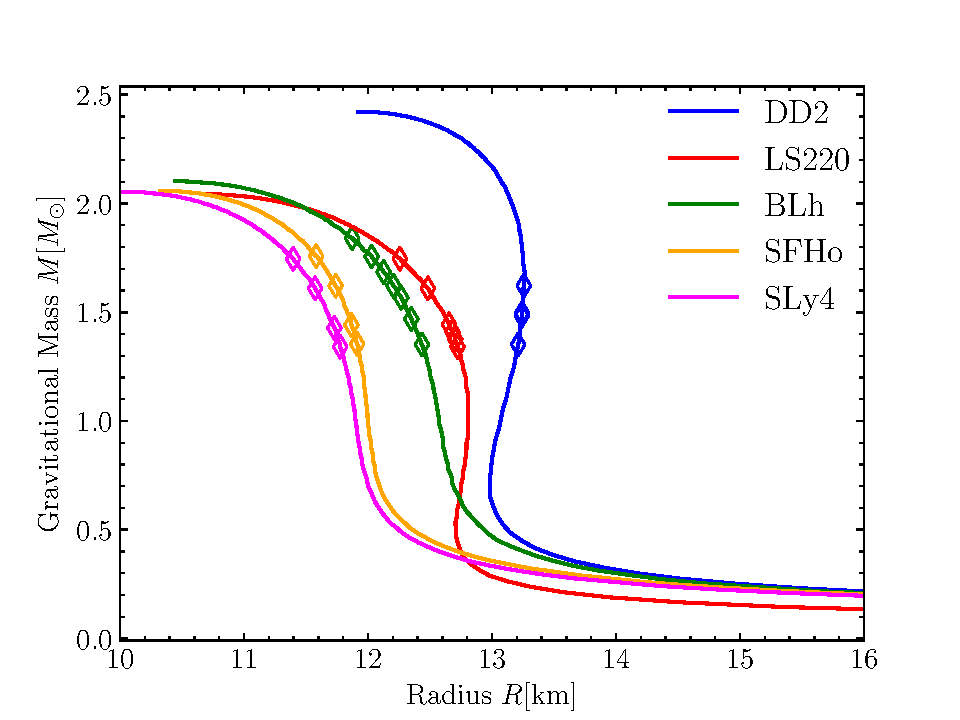
\includegraphics[width=0.49\textwidth]{tov_mr.pdf}
    \caption{Mass-radius relations for the EOSs used in this work. 
        Markers along the sequences indicate the NSs smulated in this work.}  
    \label{fig:method:tov_mr}
\end{figure}
%% 
To characterize these \acp{EOS}, that employs very different microphyscis and finite 
temperature properties and their relation to the electron fraction, we consider the \ac{TOV} solutions, 
presented on the Fig~\ref{fig:method:tov_mr}.
%
For cold, non-rotating \acp{NS}, these \acp{EOS} can support maximum 
masses in the range $\Mmax\sim 2.06-2.10\Msun$, while the predicted radii of a 1.4$\Msun$ 
NS lay in the range $R_{1.4}\sim 11.78-12.74$ km. 
More specifically, LS220, SFHo, SLy4, BLh and DD2 \ac{EOS} have 
$\Mmax$ of $2.04$, $2.06$, $2.06$, $2.10$ and $2.42$ $M_\odot$, and 
$R_{1.4}$ of $12.8$, $12.0$, $11.9$, $12.5$ and $13.2$ km respectively,.
%
These values are compatible, albeit in general lower, then those inferred from 
recent detection of an extremely massive millisecond pulsar \citep{Cromartie:2019kug} and with results obtained 
by the {\it NICER} collaboration \citep{Miller:2019cac,Riley:2019yda}.
Notably, \acp{EOS} that allow $R_{1.4}\gg 13$~km are currently disfavoured by both 
GW \ac{BNS} and X-ray pulsar observations \citep{Abbott:2018wiz,Miller:2019cac,Riley:2019yda}.
%
$\Mmax$ and $R_{1.4}$ related to the pressure at half saturation density \citep{Lattimer:2012nd}.
Thus we adopt the following naming convention for \acp{EOS}. Those that lead to a \ac{NS} with smaller 
radii are called "softer" and those that lead to a NS with larger radii are referred to as "stiffer" \acp{EOS}. 
Among considered, the DD2 \ac{EOS} is the stiffest, while SLy4 \ac{EOS} is the softest.

Finite temperature effects provides complimentary pressure support,
which is not sufficient to raise the maximum \ac{TOV} mass 
\citep{Kaplan:2013wra}, but can increase the radii of hot \acp{NS}.
Specifically, comparing the cold and hot ($s=2~{k_{\rm B}~{\rm baryon^{-1}}}$)
configurations, the thermal effects were shown to raise the $R_{1.4}$
by $15.6 \%$ for the LS220 EOS and $36.4 \%$ for the SLy4 EOS 
while for the BLh and the SFHo EOS the variation is $\sim 21-22 \%$.
%
Both \ac{NS} radius and maximum mass are increased if a \ac{NS} is rotating. 
For instance, at Keplerian limit, the maximum \ac{NS} mass is increased by 
$\sim 20\%$ for all \ac{EOS} models and radius by $\sim 40\%$ \citep{Bernuzzi:2020txg}. 
Naturally, rotation decreases the central density.
%
These observations highlight the importance of using full \acp{EOS} with finite-temperature effects. 

%% Thermal (and composition, see \citep{Kaplan:2013wra})
%% effects are indeed key to quantify the prompt collapse dynamics,
%% mass-shedding in the remnant and disc properties.

%%%% Moved to introduction chapter
%Unless stated otherwise, we label the \acp{NS} of the binary with subscripts $A$, $B$.
%The individual gravitational masses are indicated as $M_A$, $M_B$, 
%the baryonic masses as $M_{b~A}$, $M_{b~B}$, 
%the total mass as $M = M_A + M_B$, 
%and the mass ratio $q=M_A/M_B\geq1$. 
%%\red{perhaps the Lambda definition has to be moved to the bns-sims chapter}
%We define the quadrupolar tidal parameters as
%$\Lambda_i \equiv 2/3\, C_i^{-5} k^{(2)}_i$
%where $k_i^{(2)}$ is the dimensionless gravitoelectric Love number \cite{Damour:2009vw}, 
%$C_i \equiv GM_A/(c^2R_A)$ the compactness parameter, and $i=A,B$.
%The reduced tidal parameter \cite{Favata:2013rwa} is:
%\begin{equation}
%\tilde\Lambda = \frac{16}{13}\frac{(M_A+12 M_B)M_A^4 \Lambda_A}{M^5}+(A\leftrightarrow B)\,.
%\label{eq:nr_methods:Lambda_tilde}
%\end{equation}
%We use CGS units except for masses and velocities, given in units of $\Msun$ and $c$, respectively.


\section{Neutrino Radiation Transport}\label{sec:nr_methods:neut}

\red{Eq. for Q is needed as it is referenced in the results in Nu-wind}

During the neutron star mergers, the thermodynamic conditions are such that the powerful 
neutrino bursts can originate from the hot and shock heated NS matter \citep[\eg][]{Sekiguchi:2011zd}.
At high densities and temperatures reaching several MeV, the weak interaction become increasingly important,
moving the material away from the original chemical equilibrium with respect to the 
$\beta$-processes, and emission of numerous neutrinos with neutrino luminosity 
reaching $\sim10^{53}$erg s$^{-1}$ commences. 
% It was believed that such strong neutrino flux can power a \ac{GRB}, 
% however the baryon pollution of the polar region found in BNS simulations might make it 
% difficult \red{[refs, i think it was Perego work]}.

Neutrino transport is of prime importance for shaping the composition of the ejecta
\citep{Wanajo:2014wha,Sekiguchi:2015dma,Foucart:2015vpa,Foucart:2015gaa},
affecting the nucleosynthesis in the ejecta \citep{Wanajo:2014wha,Goriely:2015fqa} 
and the thermal electromagnetic counterpart, Kilonova (Macronova) \citep{Metzger:2014ila,Lippuner:2015gwa}

%%%% -----------------------------------------------------
%%%%         Introduction and Broad discussion  (From David and Others)
%%%% -----------------------------------------------------
%Neutrino interactions depend on the matter composition, its density and temperature, and on the neutrino energies. 
%For instance, at rest-mass density $10^{12}$\gcm and temperature $\sim10$~MeV, 
%the neutrino scattering on matter becomes so efficient, that they fall into the thermal equilibrium with it. 
%The mean free path of these neutrinos becomes of order of $\sim 50$~m. 
%These neutrinos are considered \textit{trapped}.
%At low densities, $<10^{11}$~\gcm, neutrinos with energy $<10$~MeV are no longer coupled to matter 
%and their mean free path can reach tens of kilometers. 
%Such neutrinos are considered \textit{free-streaming}.
%If there is a sharp density gradient present, \eg, a surface of a neutron star where density falls 
%by several orders of magnitude, then the neutrinos can be effectively divided into trapped and free-streaming. 
%The transition region, however, is more difficult to treat and requires more accurate neutrino treatment.
%%\textit{e.g.,} Monte Carly methods for solving Boltzmann equations \cite{Abdikamalov:2012zi}. Another alternative is the approximate, "ray-by-ray" \cite{Scheck:2007gw} multi-energy-group neutrino schemes [\textit{e.g.,} multi-group fluxlimited diffusion \cite{Mezzacappa:1993gn} and isotropic diffusion source approximation \cite{Liebendoerfer:2007dz}].
%
Radiation-transport equations are complex and expensive to solve numerically. 
%The main reasons for that are the following. First, is the high dimensionality of the problem. 
Radiation carriers are described by their location in space, which generally is comprised of $3$D space, momenta, 
which requires $2$ additional components, angles, and finally one component for energy of the carrier. 
Thus, with an addition of time there are $(6+1)$ dimensions for the problem. 
In addition, radiation transport depends strongly on the optical depth of the medium. 
If the latter is high, \ie, the opacity is very large, the radiation transport 
can be described by the diffusion of carriers, the formalism that have parabolic character. 
However, if the opacity is small and thus the optical depth, the radiation can stream freely, 
displaying a hyperbolic character of the transport \citep{Mihalas:1984}. 
%A particular difficulty is presented by the intermediate regime, when the radiation transport 
%mechanism transitions from diffusion to free streaming. 
%
Most commonly used approaches to simplify the radiation transport relies on reducing the diemnsionality
of the problem. In particular, -- reduce the number of spatial dimensions by assuming a certain symmetry.
%Examples are axial or spherical symmetry. And while this have shown to be a reasonable approximation for many astrophysical models, in cases where the system itself does not exhibit any spatial symmetries, 
%such simplification cannot be done. 
%%
Anther approach is to simplify the momentum space. 
%An example of such approach, that allows to reduce the computational cost considerably, is the approximation of transport equations with diffusion equations \citep{Pomraning:1973,Roe:1981}. 
%And while in the opaque regions (with high optical depth) this approximation is reasonable, it becomes much less 
%so in the transparent regions where the anisotropy of radiation has to be taking into account \citep{Ott:2008jb}.
%There, the free-streaming approximation is usually adopted. 
%%
%The solution in the intermediate region then obtained by the interpolating between the two. This approach can be augmented by using a two-moment schemes with analytic closures \citep[\eg][]{Brunner:2002}.
%However, in many applications a solution in all $(6+1)$ dimensions is a requirement.
%
%
The main source of complexity in the radiation transport stems from the scattering 
integral over all 4$\pi$ steradian.
By dividing the solid angle into a number of discrete angular intervals (rays), the integral can be replaced with a
finite sum, converting the integrodifferential equation into a linear system of equations for a multi-index object. 
%%
%This method of solving transport equation along several directions in each spatial zone the is called 
%discrete-ordinate ($S_n$) method \citep{Castor:2004,Ott:2008jb,Sumiyoshi:2012za,Godoy:2012}. 
%The discretization, however, comes with a a serious drawback, as it introduces regions which the 
%radiation cannot reach between the grid directions. 
%This is so-called "ray-effect" \citep{Morel:2003}, that causes large spatial oscillations in the transport variables.
%%
%\red{This method is a direct solution to Boltzmann eq}
%
%%A more physically motivated approximation to the radiation transport can be achieved by expending the radiation
%%It allows to convert the integrodifferential equation into a hyperbolic system of partial differential equations 
%%for the expansion coefficients. 
%%%
%%Coefficients stand for angular moments in the basis of spherical harmonic functions. 
%%An advantage of this method with respect to the diffusion approximation is that if in the latter 
%%the radaition propagation speed is unbound, in $P_N$ method, that approximates the radiation as a set of elementary
%%waves, the propagation speed is limited by the speed of light \citep{McClarren:2008b}.
%%%
%%This approach is also numerically more favorably, exhibiting the formal spectral convergence 
%%to the true solution and requiring less memory, a factor of two with respect to $S_N$ method for an 
%%equivalent angular distribution and accuracy. Preserving the rotational invariance, the $P_N$ method 
%%allows to avoid the "ray effect" of $S_N$ method. However, approximation of the radiation field with smooth 
%%basis functions, while being sufficiently accurate in the optically thick regime, displays non-physical 
%%oscillations in the transparent one \footnote{This is related to the so-called Gibbs phenomenon \cite{Boyd:2001}}.
%%If radiation is coupled to matter, these oscillations can produce regions with negative radiation intensity and 
%%thus negative temperature \citep{McClarren:2008b,Olson:2009} 
%%%
%%(see also \citet{Olson:2000,Olson:2009,Brunner:2001,McClarren:2010,Olson:2012,Hauck:2010}). 
%%%
%%One of the solutions to this problem is to filter out (using \eg, spherical spline expansion \citep{Boyd:2001}) 
%%these oscillations from the radiation intensity \citep{McClarren:2010}. However, the exact choice of the 
%%filtering technique, extension to full $3$D and absence of the clear continuum 
%%limit\footnote{Which does not allow to study the spatial convergence of the solution} 
%%present additional challenge in implementing the filtering approach. 
%
%
%Several methods are currently employed to study the neutrino radiaiton in 
%\ac{CCSN}, \ac{BNS} mergers and resulted \ac{BH}-torus systems.
%
%\begin{enumerate}
%    % ---
%    \item The simplest method to account for heating, cooling and deleptonization by neutrinos while not 
%    considering them directly, is to employ the \textbf{local source terms}, that describe the aforemntioned 
%    processes as functions of local thermodynamic quantities. This method was used in studes of shock-revival problem
%    in \ac{SN} \citep[\eg][]{Nordhaus et al., 2010; Hanke et al., 2011} and \ac{BNS} mergers \citep{Lee et al. (2005); Shibata et al. (2007)}.
%    % ---
%    \item A method that offers the simplicity of the 1 but also accounts for the optical depth of matter 
%    and geometry is the \textbf{leakage scheme} \citep{Ruffert et al. (1996); Rosswog \& Liebendorfer (2003); Kotake
%        et al. (2004); Sekiguchi (2010); O'Connor \& Ott (2010)}
%    It employs reasonable approximation to radiation transport is to consider the 
%    instantaneous energy loss via neutrino emission and evolution of the composition of the nuclear matter.
%    Neutrino leakage scheme was first proposed by \citet{vanRiper:1981mko} 
%    to study the neutrino cooling through weak interaction in the \ac{CCSN}.
%    Neutrino leakage scheme is popular to model neutrino effects in \acp{CCSN} and compact object mergers.
%    %
%    The scheme allows to estimate the effect of neutrino radiation transport, specifically tracking the 
%    evolution of the local lepton number and the association energy loss via neutrino radiation.
%    It has an advantage of being computationally efficient.
%    % ---
%    \item A more sophisticated method, that preserves the energy conservation, is the \textbf{flux-limited diffusion}
%    method. It has been widely adopted for \ac{CCSN} models of various dimensionalty and compelxity 
%    \citep{Bruenn et al., 1978; Bruenn, 1985)}.
%    The scheme's strengths include accuracy in the optically thick regions, computational efficiency and 
%    formulation, that hides the complexity of the underlying Boltzmann equation. 
%    However, by design, it relies on the specific way the transition to the optically thin regions is handled. 
%    Specifically, on the flux-limiting interpolation functions that prevent fluxes becoming superluminal. 
%    For \ac{BNS} mergers, a variant of this scheme, the multi-group (\ie, spectral) flux-limited diffusion 
%    was used by \citet{Dessart et al., 2009}.
%    % ---
%    \item In an attempt to tackle the problem of the radiation transport in different environments, the 
%    \textbf{isotropic diffusion source approximation} was derived \citep{Liebendorfer et al. (2009)}. 
%    The method splits the radiation field into the trapped part, treated via equilibrium-diffusion method, and 
%    a free-streaming part.
%    % ---
%    \item More accurate, \textbf{Boltzmann solvers}, are considerably more computationally expansive. 
%    As of now, their use is limited t othe so-called ray-by-ray approaches, that reduce the dimensionality 
%    of the problem, but may result in numerical artifacts. 
%    For instance, the state-of-the-art code for the \ac{CCSN} in 2D utilizes the ra-by-ray-plus method, where 
%    only the first two moments of the specific inteisty, (the energy denty and the flux desntiy) are evoloved.
%    This is so-called two-moment transport scheme \citep{Muller et al., 2010}.
%    Current state-of-the-art codes for the \ac{BNS} mergers also employ variations of two moment transport schemes 
%    \cite[\eg][]{Sekiguchi:2015dma}.
%    % ---
%    \item \textbf{Monte Carlo} is another way to solve the multidimensional radiation transport 
%    \citep{Fleck:1971,Gentile:2009,Abdikamalov:2012zi}. 
%    It can achieve very high accuracy, however, plague by the statistical noise 
%    (due to finite sampling of the phase space), they require very large number of Monte Carlo particles, 
%    and thus, they are computationally expensive. 
%\end{enumerate}
%%%% ---------------------------------------------------------------------------------


%% ---------------------------------------------------------
%% I N T R O  F R O M  J U S T  T H E S I S
%% ----------------------------------------------------------
%\paragraph{The equation of radiative transfer in the comoving frame}
%
%%% From Just PhD thesis
%
%Both, equations of \ac{HD} and for radiative transfer originate from \ac{BTE} for the respective frame
%independent particle distribution function \mathcal{F}, defined as 
%
%\begin{equation}
%    \dd N = \frac{g}{h^3}\mathcal{F}(\boldsymbol{x},\boldsymbol{p},t)\dd \boldsymbol{x} \dd \boldsymbol{p}
%\end{equation}
%
%where $\dd N$ is the number of particles in the phase space-space $\dd\boldsymbol{x}\dd\boldsymbol{p}$,
%$g$ is the statistical weight of the species and $h$ is the Plank's constant. 
%Under the ``radiation'', in this context, is implied the specific distribution of particles that move with the 
%speed of light and that are not influenced by external forces $\dot{\boldsymbol{p}}=0$.
%The \ac{BTE} in the fixed frame reads 
%
%\begin{equation}
%    \frac{1}{c}\frac{\partial}{\partial t} \mathcal{F} + \boldmath{n}\cdot\nabla_{x}\mathcal{F} = B,
%    \label{eq:theory:bte}
%\end{equation}
%
%where $\boldsymbol{n} = \boldsymbol{p}/|\boldsymbol{p}|$ and $B = B(\boldsymbol{x},\boldsymbol{p},t)$ 
%is the ``collision integral'' that in general has seven dimensions and includes explicit integrals in
%momentum space. Thus, Eq.~\eqref{eq:theory:bte} is the integro-partial differential equation.
%The quantity that is often used to discuss the frame dependent specific (\ie, monochromatic) intensity, 
%
%\begin{equation}
%    \mathcal{I}(\boldsymbol{x},\boldsymbol{n}, \epsilon, t) = (\epsilon/hc)^3 c \mathcal{F}(\boldsymbol{x},\boldsymbol{p},t)
%    \label{eq:theory:intensity}
%\end{equation}
%
%where $\epsilon = |\boldsymbol{p}|c$ is the energy. 
%Generally, the specific intensity $\mathcal{I}$ is measured in the frame comoving with the fluid, as the 
%collision integral, $B$, depends primarily on the particle distribution of the fluid part of the system.
%This is motivated by the fact that under the \ac{LTE}, the fluid distribution function becomes isotropic. 
%The symmetries allow to simplify the collision integral and makes it calculation more numerically 
%advantageous.
%%
%Next, we introduce the comoving-frame equation of radiation transport up to order 
%$\mathcal{O}(\upsilon/c)$ where $\upsilon=|\boldsymbol{\upsilon}|$ is the velocity of the fluid 
%measured in the lab frame. The laboratory or ``lab frame'' is a frame constructed from arbitrary but 
%fixed Eulerian coordinates. The equations read 
%\citep[\eg][]{Buchler, 1979; Kaneko et al., 1984; Munier & Weaver, 1986}
%
%\begin{equation}
%    \begin{aligned}
%    \frac{1}{c}\frac{\partial\mathcal{I}}{\partial t} + \frac{\boldsymbol{\upsilon}\cdot\boldsymbol{n}}{c^2}\frac{\partial\mathcal{I}}{\partial t} + n^j\frac{\partial\mathcal{I}}{\partial x^j} + \frac{\upsilon^j}{c}\frac{\partial\mathcal{I}}{\partial x^j} + \frac{\partial}{\partial \epsilon}\Big[ \mathcal{I}\epsilon \Big( \frac{\boldsymbol{a}\cdot\boldsymbol{n}}{c^2} + \frac{1}{c} n^j n^k \nabla_j\upsilon_k \Big) \Big] \\
%    + \frac{\partial}{\partial n^i}\Big[ \mathcal{I} \Big( \frac{\boldsymbol{a}\cdot\boldsymbol{n}}{c^2}n^i - \frac{a^i}{c^2} + \frac{1}{c}n^in^j\nabla_j\upsilon_k - \frac{1}{c}n^j\nabla_j\upsilon^i - k^i_{jk}n^jn^k - \frac{1}{c}\Gamma^{i}_{jk}\upsilon^j n^k \Big) \Big] \\
%    + \mathcal{I} \Big[ 2 \frac{\boldsymbol{a}\cdot\boldsymbol{n}}{c^2} \frac{1}{c}\nabla_i\upsilon^i + \Gamma^i_{ij}n^j + \frac{1}{c}n^i n^j\nabla_i\upsilon_j \Big] = C,
%    \end{aligned}
%    \label{eq:theory:bte_full}
%\end{equation}
%
%where $\boldsymbol{a} = \partial_t \boldsymbol{\upsilon}$, $\Gamma^i_{jk}$ are 
%Christoffel symbols associated with the spatial coordinates and $C = (\epsilon/hc)^3 c B$.
%Equation Eq.~\eqref{eq:theory:bte_full} can be obtained from Eq.~\eqref{eq:theory:bte}, using 
%Eq.~\eqref{eq:theory:intensity} and the $\mathcal{O}(\upsilon/c)$ variant of the Lorentz 
%transformations for $\mathcal{I}$, $\epsilon$, and $\boldsymbol{n}$.


\subsection{Neutrino leakage scheme}

\red{Introduce electron fraction, \&
beta equilibrium condition
}

\begin{table}
    \caption{
        Weak reactions employed in our simulations and references for their implementation.
        In the left column, $\nu \in \{\nu_e, \bar{\nu}_e, \nu_{x}\}$ denotes any neutrino species, 
        $\nu_{x}$ any heavy-lepton neutrinos, $N \in\{n, p\}$ a nucleon, and $A$ any nucleus.
        In the central column the role of each reaction is highlighted with "P" standing for 
        production, "A" for absorption opacity and "S" for scattering opacity.
        When two roles are included, the second refers to the inverse ($\leftarrow$) reaction.
        Table is taken from \citet{Radice:2018pdn}.
    }
    \label{tab:leakage}
    \begin{center}
        \begin{tabular}{l l l}
            \hline\hline
            Reaction & Role &  Ref. \\ 
            \hline
            $p + e^- \leftrightarrow \nu_e + n $          & P,A & \citep{Bruenn:1985}  \\
            $n + e^+ \leftrightarrow \bar{\nu}_{e} + p $  & P,A & \citep{Bruenn:1985}  \\
            $e^+ + e^- \rightarrow \nu + \bar{\nu}$       & P   & \citep{Ruffert:1995fs} \\
            $\gamma + \gamma \rightarrow \nu + \bar{\nu}$ & P   & \citep{Ruffert:1995fs} \\
            $N + N \rightarrow \nu + \bar{\nu} + N  + N$  & P   & \citep{Burrows:2004vq} \\
            $\nu + N \rightarrow \nu + N$                 & S   & \citep{Ruffert:1995fs} \\
            $\nu + A \rightarrow \nu + A$                 & S   & \citep{Shapiro:1983du} \\
            \hline\hline
        \end{tabular}
    \end{center}
\end{table}

For numerical reasons, the neutrino transport in the optically thick region, 
where radiation and matter are coupled, is handled the so-called ``leakage scheme''. 
The method accounts for the optical depth of matter and geometry 
\citep{Ruffert:1995fs,Rosswog:2003rv,Sekiguchi:2010zz,OConnor:2009iuz,Galeazzi:2013mia}
%
For other implementations and methods see \eg, 
\citet{vanRiper:1981mko,Ruffert:1995fs,Rosswog:2003rv,OConnor:2009iuz,Sekiguchi:2010ep,
    Neilsen:2014hha,Perego:2015agy,Ardevol-Pulpillo:2018btx}.
%
The method approximates the radiation transport evaluating the instantaneous energy loss 
via neutrino emission and evolution of the composition of the nuclear matter.
The particular advantage of the method is its computational efficiency and an ability 
to account for non-trivial geometries of emitting regions.
%
It was first proposed by \citet{vanRiper:1981mko} to study the neutrino cooling through weak interaction 
in the \ac{CCSN}. The leakage scheme is popular to model neutrino effects in \acp{CCSN} 
and compact object mergers.
%
A modified version of \citet{Galeazzi:2013mia} scheme is implemented in 
\ac{NR} code \wisky{} \citep{Radice:2016dwd,Radice:2018pdn}.

%Non-equilibrium weak-interaction processes lead to the production of numerous neutrions 
%from the hot, dense and neutron-rich matter, \textit{e.g.,} BNS merger remnant. 
%The cooling effect associated with the neutrino emission, that could cause dynamical 
%instabilities, is important for the structure and evolution of the remnant. 
%To evaluate the influence of thermal effects on the onset of dynamical instabilities, the long-term evolution, (several dynamical timescales of the object with $M$ mass and $R$ size $\tau_{\text{dyn}}\sim(M/R^3)^{1/2}\approx 1$~ms) is required.

%
The goal of the scheme is to describe a series of effective emissivities, 
$R_{\nu}^{\text{eff}}$, and $Q_{\nu}^{\text{eff}}$ for electron neutrinos, $\nu_e$, 
anti-electron neutrinos $\bar{\nu}_e$ and the heavy-lepton neutrinos, 
which are collectively labeled as $\nu_x$.
Here $R_{\nu}^{\text{eff}}$ describes the the number of neutrinos emitted per second and baryon,
and $Q_{\nu}^{\text{eff}}$ describes the energy emitted via neutrinos per second and baryon.
%
Then, the optical depth is evaluated and used to reduce the intrinsic emissivites, 
mimicking the effect of the diffusion of radiation from the optically thick regions.
%\red{This scheme also includes the heating effects by the free-streaming neutrinos, \textit{i.e.,} neutrino absorption}. \gray{ which was shown to be important for altering the ejecta composition }.
%
%The following neutrino species are considered: electron neutrino, $\nu_e$, 
%(and its anti-neutrino $\bar{\nu}_e$) and heavy lepton neutrino $\nu_{\tau,\mu}=\nu_X$ (and its antineutrino). %\gray{that are a single component with statistical weight of 4.}.
%
Neutrinos are assumed to be massless and in thermal equilibrium with the surrounding matter.
%As a result, the energy spectrum of the neutrinos follows a Fermi-Dirac distribution for
%ultrarelativistic particles at the temperature of the matter. 
%The chemical potential $\nu_e$ and $\bar{\nu}_e$ is assumed to the at equilibrium, \cite{Rosswog:2003rv},
%
%\begin{equation}
%\mu_{\nu_e}^{\text{eq}} = \mu_e - \mu_n - \mu_p = -\mu_{\bar{\nu}_e}^{\text{eq}}
%\end{equation}
%
%where $\mu_e$, $\mu_n$, $\mu_p$ are the relativistic chemical potentials including the rest-mass of the particle. 
The $R_{\nu}^{\text{eff}}$, and $Q_{\nu}^{\text{eff}}$ can be evaluated from various 
weak-interaction processes present in the hot and dense matter of the NS. 
%The definitions are: the $Q_{\nu_{i}}$ is the energy emitted via neutrinos per second and baryon;
%the $R_{\nu_{i}}$ is the number of neutrinos emitted per second and baryon.
%%
%The most important neutrino emission processes in the NS remnant are: 
%\begin{itemize}
%    \item electron and position capture on nucleons, the $\beta$-process,
%    \item electron-positron pair annihilation, 
%    \item transverse plasmon decay.
%\end{itemize}
%
The reactions considered with in the scheme, implemented in \wisky{} are listed in the 
Tab.~\ref{tab:leakage}.
%
It is possible to evaluate the emission rates corresponding to these processes 
using only the quantities provided by the \ac{EOS} tables.

%%%% === URCA PROCESS
For instance, consider the strong neutrino emitting process, the direct Urca process, 
that consists of the $\beta$-decay, $e^+ + n \rightarrow p + \bar{\nu}_e$ 
and the electron capture on the free nucleons (n), $e^{-} + p \rightarrow n + \nu_e$ 
(the first two reactions Tab.~\ref{tab:leakage}). 
This process moves the matter to the $\beta$-equilibrium, in which the rats 
of both reactions are the same, and the chemical potentials $\mu_{\nu_e,\bar{\nu}_e}=0$.
%
For both, $\beta$-decay, ``\text{pc}'', and electron capture, ``\textit{ec}'', the 
\begin{equation}
\begin{aligned}
    Q_{pc}(\bar{\nu}_e) &= n_b^{-1}\beta\eta_{pn}T^6F_5(-\eta_e)[1-f_{\bar{\nu}_e}]_{pc} \\
    Q_{ec}(\nu_e) &= n_b^{-1}\beta\eta_{np}T^6F_{5}(\eta_e)[1-f_{\nu_e}]_{ec}
\end{aligned}
\label{eq:theory:qecpc}
\end{equation}
and
\begin{equation}
\begin{aligned}
    R_{pc}(\bar{\nu}_e) &= n_b^{-1}\beta\eta_{pn}T^5F_4(-\eta_e)[1-f_{\bar{\nu}_e}]_{pc} \\
    R_{ec}(\nu_e) &= n_b^{-1}\beta\eta_{np}T^5F_{4}(\eta_e)[1-f_{\nu_e}]_{ec}
\end{aligned}
\label{eq:theory:recpc}
\end{equation}
where $T$ is the temperature, $n$ are the number densities, $\eta=\mu/T$ with $\mu$ being the 
chemical potential, $F_N$ are the Fermi integrals of order $N$,
$1-f_{\nu}$ is a factor related to the Fermi-Dirac distribution, $f_{\nu}$, and $\beta$
is a constant \citep{Bruenn:1985}.
%
Equations Eq.~\eqref{eq:theory:qecpc} and \eqref{eq:theory:recpc} display a strong dependency 
of neutrino production on temperature.
%
%$Q_{\text{pc}}(\bar{\nu}_e),Q_{\text{ec}}({\nu_e}) \propto T^{6}$ 
%while 
%$R_{\text{pc}}(\bar{\nu}_e),R_{\text{ec}}(\nu_e)\propto T^5$, 
%
%At high temperatures but moderate densities, the plasmon decay is one of the major sources of neutrinos, 
%where the plasmon is the quanta of electromagnetic field in plasma exhibiting two polarizations, 
%among which only the tansverse polarisation is important in this context.
%\cite{P. J. Schinder, D. N. Schramm, P. J.Wiita, S. H. Margolis, and D. L. Tubbs, Astrophys. J. 313, 531 (1987).} 
%\red{But I am not sure that plasmon decay in included in the Leackage scheme on Whisky}


%%% ==== SCATTERING
In addition to the emission of neutrinos, the leakage scheme considers the neutrino absorption and scattering, 
(see "A" and "S" entries in the Tab.~\ref{tab:leakage}, $\nu+A\rightarrow\nu+A$ is the coherent neutrino 
scattering on heavy nuclei (with atomic mass number $A$), and $\nu+N\rightarrow\nu+N$ 
is the neutrino scattering on free nucleons).
%
Of particular importance are the neutrino scattering on heavy nuclei, and on free nucleons, 
as well as electron-flavor neutrinos absorption on free nucleons. 
The mathematical formulation of these opacities see \citet{Galeazzi:2013mia} and their Appendix A.
%
The neutrino scattering on nuclei becomes the dominant opacity source when the heavy neuclei 
are abundant, nuclei that form below nuclear saturation density ant low temperatures $<15$~MeV \citep{Rosswog:2003rv}.

Taking the considered scattering and absorption processes, the local mean free-path for each neutrino species 
can be computed. From it, the energy-independent mean free path can be derived, that in turn depends 
only on the local thermodynamic condition. 
This allows to evaluate the energy-independent part of the optical depth and diffusion rates.
%
The optical depth allows to asses the extend of the optically thick region 
(that is neutrino-species dependent) and it allows to asses the time needed for neutrinos to 
diffuse out of the dense matter, diffusion timescales.. 
%It should be noted that for cores of a neutron star this diffusion timescale is of order of seconds. 
%Thus, neutrinos that are expected to contribute the most on the dynamical timescale are the nuetirnos abundantly
%emitted at the \textit{neutrinosphere} and above \citep{Galeazzi:2013mia,Endrizzi:2018uwl}.
%
%\red{The diffusive number and energy emission rates per baryon are 'interpolated' 
%    between diffusive and free-streaming regimes.
%    So it seems that both, diffusion rates and free neutrino emission rates per baryon are computed here, using the ioptical depth to separate them. Then, the effective rates are computed via interpolation.
%}

%A quatity that is op particular usefullness for describing neutrino cooling  is the neutrinosphere,
%defined as \cite{Galeazzi:2013mia}
%\begin{equation}
%\frac{Q_I}{Q_{I}^F} = \frac{2}{3}
%\end{equation}
%where $Q_I$ is the interpolated effective emission rate, $Q_I^F$ is the neutrino luminosity per baryon.
%The neutrino cooling is suppressed inside this region, and the neutrino escape timescale is the diffusion timescale. 
%The neutirnosphere is however can also be defined as $\tau=2/3$, \textit{e.g.,} \cite{Rosswog:2003rv,Endrizzi:2018uwl}.
%After the interpolation, the net net emission rate per baryon appearing $\mathcal{R}$ and and the luminosity per baryon $\mathcal{Q}$.
%
%Importantly, the assumption of the chemical equilibrium can lead to an overestimation of the neutrino emission rates in the transition region, etween the optically thin and thick.

%%%%% ==== from Radice2018pdn >>>
%
%Alongside the neutrino production rate, $R_{\nu}$, and respective energy release, $Q_{\nu}$, for 
%$\nu\in\{\nu_e,\bar{\nu}_e,\nu_x\}$, the opacities, $\kappa_{\nu;a}$ and $\kappa_{\nu;s}$ 
%for absorption and scattering respectively are evaluated, where the 
%thermodynamical equilibrium chemical potential is assumed for neutrinos.
%
The opacities are split into two types. The density weighted opacities $\kappa_{\nu;a}^0$ and
$\kappa_{\nu;s}^0$ and energy density weighted opacities $\kappa_{\nu;a}^1$ and $\kappa_{\nu;s}^1$. 
The former are related to the rate at which neutrinos escape the material, 
while the latter set the rate at which energy escapes the material as neutrinos escape 
\citep{Ruffert:1995fs}.
%
The optical depth, $\tau_{\nu}^{\alpha}$ is computed taking into account 
total neutrino opacities $\kappa_{\nu;a}^j + \kappa_{\nu;s}^j$ \citep{Neilsen:2014hha}.
%
Optical depth is then used to estimate the effective emission rates \citep{Ruffert:1995fs} as 
%
\begin{equation}
R_{\nu}^{\text{eff}} = \frac{R_{\nu}}{1 + t_{\text{diff}}^0(t^0_{\text{loss}})^{-1}}
\label{eq:method:whisky:Rnueff}
\end{equation}
%
where $t_{\text{diff}}$ and $t_{\text{loss}}$ are the neutrino diffusion time and emission timescales,
%
\begin{equation}
t_{\text{diff}}^{0} = \mathcal{D}\frac{(\tau_{\nu}^0)^2}{\kappa_{\nu;a}^0 + \kappa_{\nu;s}^0}, \hspace{5mm} t_{\text{loss}}^0 = \frac{R_{\nu}}{n_{\nu}},
\end{equation}
%
%and the neutrino emission timescale 
%
%\begin{equation}
%t_{\text{loss}}^0 = \frac{R_{\nu}}{n_{\nu}}
%\end{equation}
%
and $n_{\nu}$ is the neutrino number density estimated based on the 
beta equilibrium with neutrinos and \red{$\tau_{\nu}$ is the optical depth}.
The $\mathcal{D}$ is a tuning parameter set to $6$ \citep{Radice:2018pdn}.
%
Similarly, the effective energy emission rate $Q_{\nu}^{\text{eff}}$ 
is computed with $\tau_{\nu}^1$, $\kappa_{\nu;a}^1$ and $\kappa_{\nu;s}^1$.

%Notably, the effect of trapped neutrinos was shown to be weak in the \ac{NS} conditions 
%\citep{Galeazzi:2013mia} and thus neglected here.
The neutrinos that escape according to the effective rate $R_{\nu}^{\text{eff}}$,
with the average energy $U_{\nu}^{\text{eff}}/R_{\nu}^{\text{eff}}$ 
are the free streaming neutrinos $n_{\nu}^{\text{fs}}$. 
%
These neutrinos are treated afterwards according to the 
M0 scheme in the optically thin region \citep{Radice:2016dwd}.

%% ----------------------------------
%%%% from Galezzi:2013 again
%% ----------------------------------
%Note that the total neutrino luminocity is an observer dependent quantity in relativity. 
%The reason is that the the neutrino energy emitted at a given point between coordinate times $t$ and $t+dt$, 
%which are measured by the coordinate observer with world line tangent to $t^{\mu}$. 
%Further assumption of stationarity is then required, \eg, assuming $t^{\mu}$ is the Killing vector. 
%Then, the neutrino energy at infinity is $E_{\nu}^{\infty} = \sqrt{-g_{00}}E_{\nu}$, 
%irrespective of the direction of emission.
%
%Summarizing, since (trapped) neutrinos are assumed to be in equilibrium with the baryonic matter, the number density and energy distribution of neutrinos is not evolved -- their contribution to the source terms 
%$\Psi^{\beta}$ 
%$Qu^{\mu}$ and 
%$N$ 
%$R_{p,n}$
% is obtained from the matter properties.

%\gray{only the electron neutrinos are considered there, and only their degrees of freedom is accounted for by the electron fraction $Y_e=n_e/n_b$.
%    The electron fraction is changed only by the neutrinos (antineutrinos) according to the source term $N$.}

%\gray{Galezzi:13:
%    pressure and specific internal energy contain contributions of baryons, electrons, photons and trapped neutrinos
%    \begin{align}
%    p &= p_e + p_b + p_{\gamma} + p_{\nu_e,\bar{\nu}_e}... \\
%    \epsilon &= \epsilon_e + \epsilon_b + \epsilon_{\gamma} + \epsilon_{\nu_e,\bar{\nu}_e} + ...
%    \end{align}
%    where the contribution from trapped electron-neutrinos $\nu_e$ and
%    antineutrinos $\bar{\nu}_e$ in the dense baryonic component can be evaluated from the thermodynamic state of the fluid and assuming that the neutrinos are following a Fermi-Dirac distribution 
%    \begin{align}
%    p_{\nu_e,\bar{\nu}_e} &= p_{\nu_e} + p_{\bar{\nu}_e} = \frac{4\pi}{3}T^4[F_3(\eta_{\nu_e}) + F_3(\eta_{\bar{\nu}_e})], \\
%    \epsilon_{\nu_e,\bar{\nu}_e} &= \epsilon_{\nu_e} + \epsilon_{\bar{\nu}_e} = \frac{1}{3}\frac{p_{\nu_e,\bar{\nu}_e}}{\rho}
%    \end{align}
%    where $\eta_{\nu_e} = \mu_{\nu_e}/T$ and $\eta_{\bar{\nu}_e} = \mu_{\bar{\nu}_e}/T$ are the degeneracy parameters for the electron-neutrinos and antineutrinos, $\mu_{\nu_e}$, $\mu_{\bar{\nu}_e}$ the corresponding chemical potentials and $T$ is the temperature, $F_3(\eta_{\nu_e})$ is the Fermi integral.
%    There, the contributions of trapped neutrinos to pressure and internal energy is neglected, 
%    $p_{\nu_{e},\bar{\nu}_e}=\epsilon_{\nu_e,\bar{\nu}_e}=0$.
%    For the computation of the neutrino source term $N$, the neutrinos emission rates per baryond are introduced $R_{\nu_e}$ and $R_{\bar{\nu}_e}$ for electron neutrinos and antineutrinos respectively. Then in the fluid rest-frame the change in electrom fraction is $u^{\alpha}\nabla_{\alpha}(Y_e)=\matcal{R} = R_{\bar{\nu}_e} - R_{\nu_e}$. 
%    Similarly, for the source term $\Psi^{\beta}$ that describes the radiative losses of energy and momentum due to neutrinos, the neutrino emissivity $Q$ is intorcued. Assumptions: emission is isotropic in the fluid's rest frame. Then the covarient equation reads 
%    \begin{equation}
%    \Psi^{\beta} = -\rho m_b^{-1}Qu^{\beta} = \rho m_b^{-1}\sum_I Q_I u^{\beta} = -\rho m_b^{-1} (Q_{\nu_e} + Q_{\bar{\nu}_e} + Q_{\nu_{\tau,\mu}}+Q_{\bar{\nu}_{\tau,\mu}})u^{\beta}
%    \end{equation}
%    Here, the emissivity due to the $\tau$ and $\mu$ neutrinos into a single contribution $ Q_{\nu_{\tau,\mu}}$.
%    These equations, for numerical evolution, the equations are cast into a flux conservative formulation, based on the Valencia formulation, representing Eurler equtions and lepton/baryon number conservations as balance laws.
%    \begin{equation}
%    \partial_t (\sqrt{\gamma}\boldsymbol{q}) + \partial_t\Big( \sqrt{\gamma} \boldsymbol{f}^{(i)}(\boldsymbol{q}) \Big) = s(\boldsymbol{q}).
%    \end{equation}
%    where $\gamma$ is the determinant of the three-metric, while $\boldsymbol{f}^{(i)}(\boldsymbol{q})$ and $s(\boldsymbol{q})$ are the flux vectors and source terms, respectively \cite{Font:2008fka}.
%}

%The foundation of the scheme described here is presented in \cite{Galeazzi:2013mia}.
%The method is similar to that of the \cite{Ruffert:1995fs}.
%And, as in the \cite{Rosswog:2003rv}, the opacities are computed on the basis local thermodynamical equilibrium chemical potential for the neutrinos.


%The scheme consideres three neutrino species: electron neutrino $\nu_e$, electron antineutrino $\bar{\nu}_e$ and an single species $\nu_x$ for heavy-lepton neutrinos.
%The reactions traced by the scheme are listed in the table \ref{tab:leakage}.



%\gray{
%    Notably, the $E == n_{\alpha}n_{\beta}T^{\alpha\beta}$, 
%    $S_i = -\gamma_{i\alpha}n_{\beta}T^{\alpha\beta}$ and $S_{ij} = \gamma_{i\alpha}\gamma_{j\beta}T^{\alpha\beta}$ are the matter source terms where $n_{\alpha}=(-\alpha, 0, 0, 0)$ is the future pointing four-vector orthonormal to the space-like hypersurface, $S=S_{i}^{i}$ is the trace.
%}






\subsection{Neutrino M0 scheme}

%% === From Just thesis
%In order to describe the interaction of free-streaming neutrinos effects with matter a variant of the 
%Boltzmann solver is required. In the following we consider a particular technique, 
%commonly referred to as a variable Eddington factor technique, that is based on the evolution 
%of the set number of moments of the specific intensity. 
%For instance, if the number is two, namely, the
%energy density and flux density are evolved, such scheme is called two-moment transport scheme.
%There the second moment, the Eddington factor is obtained in a separate procidure via solving 
%the simplified Boltzmann equation \citep{(e.g. Mihalas & Mihalas, 1984)}.
% -------------------------

The free-streaming neutrinos are treated via a variant of the moment equations of energy transport, 
the M0 scheme \citep{Radice:2016dwd,Radice:2018pdn}.
Computation of the neutrino number density and energy is 
%$n_{\nu_e}$, $n_{\bar{n}_e}$, $E_{\nu_e}$ and $E_{\bar{\nu}_e}$ is 
accomplished via the zeroth momentum (M0) of the free-streaming neutrino distribution 
function on a set of individual radial rays, with the closure adopted to the post-merger geometry.

%% M0 Appendix A from Radice:2016dwd, Neutrin transport details
%\subsubsection{The Boltzmann equations for Free-Streaming Neutrinos}
%First, the Boltzmann equation is derived for the neutrinos, that are again assumed to be massless 
%particles. 
Neutrinos propagate in the fluid with four-velocity is $u^{\alpha}$ and four-momentum, $p^{\alpha}$.
The latter can be decomposed as \citep{Thorne:1981}
%
%% \begin{equation}
$p^{\alpha} = (-p_{\beta}u^{\beta})(u^{\alpha} + r^{\alpha})$, 
%% \end{equation}
%
where $E_{\nu}=-p_{\alpha}u^{\alpha}$ is the neutrino energy measured by Eulerian observer,
comoving with the fluid, $r^{\alpha}$ is the unit space-like vector, orthogonal to the 
fluid's $u^{\alpha}$, or in other words $r_{\alpha}r^{\alpha}=1$ and $u_{\alpha}r^{\alpha}=0$.
%
Additionally, $r^{\alpha}$ can be interpreted as the direction along which neutrinos move,
as seen by the Eulerian observer comoving with the fluid.
%
The four-vector of the neutrinos is
%
%% \begin{equation}
%% \label{eq:method:whisky:neut:k}
$k^{\alpha} = u^{\alpha} + r^{\alpha}$ 
%% \end{equation}
%
with $k_{\alpha}k^{\alpha} = 0$ normalized such that $k^{\alpha}u_{\alpha}=-1$.
%
Next, the affine parameter, $l$, that parameterizes the neutrino's worldline is introduced
%
%% \begin{equation}
%% l = \int (-p_{\alpha u^{\alpha}})\dd s \text{ so that } \Big( \frac{\partial}{\partial l} \Big)^{\alpha} = %% k^{\alpha}.
%% \end{equation}
% 
such that $(\partial / \partial l)^{\alpha} = k^{\alpha}$.
%
Now, with $l$, the Boltzmann equations for the neutrino radiation transport read \citep{Thorne:1981}
%
\begin{equation*}
\frac{D F}{D l} = \mathbb{C}[F],
\end{equation*}
%
where $F$ is the distribution function for a give neutrino species, and $\mathbb{C}$ is the
``collisional operator'' that contains information regarding the interactions 
between neutrinos and the background fluid (in the frame of the fluid. 
%
The $D/Dl$ is the total derivative in phase space along $p^{\alpha}$ and it reads 
%
\begin{equation}
\label{eq:method:whisky:neut:bolzeq}
\frac{DF}{Dl} = k^{\alpha} \Big[ \frac{\partial F}{\partial x^{\alpha}} - \Gamma^{\delta}_{\:\:\alpha\beta}p^{\beta}\frac{\partial F}{\partial p^{\delta}} \Big],
\end{equation}
%
where $\Gamma^{\delta}_{\:\:\alpha\beta}$ are the Christoffel symbols.
%
%\subsubsection{Neutrino number density evolution}
%Neutrinos are split into two categories. 
%Trapped neutrinos are treated with leackage scheme.

The obtained Boltzmann equation, Eq.~\eqref{eq:method:whisky:neut:bolzeq}, allows to describe
the evolution of the free-steaming neutrinos and track the evolution of their average energy.
%
The source term is computed taking the effective emissivities from the leakage scheme.
The collisional term is approximated in a way that it only includes neutrino absorption and emission. 
Scattering is neglected.
For the evaluation of the absorption opacities, (of $\nu_{e}$ and $\bar{\nu}_{e}$) the 
\ac{LTE} is assumed.
The neutrinos are assumed to propagate along the radial rays. 
\citep{Radice:2016dwd,Radice:2018pdn}.

%%%% ---------------------------
%% On the Balance Eqution and Closure
%%%% ---------------------------
%The neutrino number density (in the fluid rest frame) for neutrinos of a give flavor, $n_X$, 
%can be expressed through the neutrino number current $J_{X}^{\alpha}$ that reads \citep{Lindquist:1966},
%%
%\begin{equation}
%J_{X}^{\alpha} = \int F p^{\alpha} \frac{\dd^3 p}{-p_0}
%\end{equation}
%%
%as $n_X = - u_{\alpha} J_{X}^{\alpha}$.
%%
%The balance equation (between absorption and emission of neutrinos) can be obtained from the 
%first moment of the Boltzmann equation \cite{Thorne:1981,Shibata:2011kx}
%%
%\begin{equation}
%\label{eq:method:whisky:neut:balanseq}
%\nabla_{\alpha}J_{X}^{\alpha} = R_{X}^{\text{eff}} - \kappa_X n_X,
%\end{equation}
%%
%where $\kappa_X$ is the absorption opacity and $R_X^{\text{eff}}$ is the effective neutrino emission rate.
%%
%While the equation Eq.~\eqref{eq:method:whisky:neut:balanseq} is exact, in order to be solved, 
%it requires closure. 
%In this method the closure is given by considering neutrinos only 
%propagating radially and at a speed of light, \eg, 
%%
%%% \begin{equation}
%$J_{X}^{\alpha} = n_X k^{\alpha}$, 
%%% \end{equation}
%%
%where $k^{\alpha}$ is the fiductial null vector from 
%$k^{\alpha} = u^{\alpha} + r^{\alpha}$ %% \eqref{eq:method:whisky:neut:k}, 
%under the assumption that $r^{\alpha}$ is the radial null-vector, orthogonal to the fluid $u^{\alpha}$.
%%This translates into the assumption that the free-streaming neutrinos are 
%%moving radially in a frame instantaneously comoving with the fluid.
%%
%Then, the balance equation for $n_X$ reads
%%
%\begin{equation}
%\label{eq:mehtod:whisky:neut:balanseq2}
%\partial_t(\sqrt{-g}n_X k^t) + \partial_r(\sqrt{-g}n_X k^r) = \sqrt{-g}(R^{\text{eff}}_{X} - \kappa_X n_X)
%\end{equation}
%%
%where $g$ is the determent of the $4$-metric \gray{(in spherical coordinates)}.
%%%% -------------------------------------

The balance equation (between absorption and emission of neutrinos) can be obtained from the 
first moment of the Boltzmann equation \citep{Thorne:1981,Shibata:2011kx}
%\begin{equation}
%\label{eq:theory:neut:balanseq1}
%\nabla_{\alpha}J_{X}^{\alpha} = R_{X}^{\text{eff}} - \kappa_X n_X,
%\end{equation}
%\begin{equation}
%\label{eq:theory:neut:balanseq1}
%\partial_t(\sqrt{-g}n_X k^t) + \partial_r(\sqrt{-g}n_X k^r) = \sqrt{-g}(R^{\text{eff}}_{X} - \kappa_X n_X)
%\end{equation}
%
%where $n_X$ is the number density, 
%$\kappa_X$ is the absorption opacity and $R_X^{\text{eff}}$ 
%is the effective neutrino emission rate.
%
The closure is achieved by considering neutrinos propagating only radially with the 
speed of light, $\partial_t$ is a Killing vector. 
Then the free-streaming neutrino energy satisfies \cite{Radice:2016dwd,Radice:2018pdn}.

\begin{subequations}
    \begin{align}
        \partial_t(\sqrt{-g}n_X k^t) + \partial_r(\sqrt{-g}n_X k^r) &= \sqrt{-g}(R^{\text{eff}}_{X} - \kappa_X n_X) \label{eq:theory:neut:balanseq1} \\
        k^t\partial_t(E_{\nu}^{\text{fs}}\chi) + k^r\partial_r(E_{\nu}^{\text{fs}}\chi) &= \frac{\chi}{n_{\nu}^{\text{fs}}} (Q_{\nu}^{\text{eff}} - E_{\nu}^{\text{fs}}R_{\nu}^{\text{eff}}) \label{eq:theory:neut:balanseq2} 
    \end{align}
\end{subequations}

where $n_X$ is the number density, $\chi=-k^{\alpha}(\partial_t)_{\alpha}$
$\kappa_X$ is the absorption opacity and $R_X^{\text{eff}}$ 
is the effective neutrino emission rate.

%\begin{equation}
%\label{eq:theory:neut:balanseq2}
%\partial_t(\sqrt{-g}n_X k^t) + \partial_r(\sqrt{-g}n_X k^r) = \sqrt{-g}(R^{\text{eff}}_{X} - \kappa_X n_X)
%\end{equation}
%
%\begin{equation} %% Eq 9 from 2018pdn
%    \label{eq:theory:neut:balanseq2}
%    k^t\partial_t(E_{\nu}^{\text{fs}}\chi) + k^r\partial_r(E_{\nu}^{\text{fs}}\chi) = \frac{\chi}{n_{\nu}^{\text{fs}}} (Q_{\nu}^{\text{eff}} - E_{\nu}^{\text{fs}}R_{\nu}^{\text{eff}})
%\end{equation}
%
%
%The equation Eq.~\ref{eq:theory:neut:balanseq2} is then solved 
%numerically on a series of 
%independent radial rays at every timestep of the evolution.

%%%% --------------------------------------------
%% Neutrino average energy evolution
%%%% --------------------------------------------
%Next, the computation of the neutrino average energy is 
%required to evaluate the matter composition and temperature changes.
%%
%Here the additional assumption is made, that the space-time is stationary, \eg, 
%$t^{\alpha}:=(\partial_t)^{\alpha}$ is a Killing vector, which leads to the 
%$(-p_{\alpha}t^{\alpha})$ to be a conserved quantity.
%%
%% Assuming that there is no interaction with the fluid and the along the neutrino worldlines, \eg, 
%%
%%% \begin{equation}
%%% $\frac{\dd(-p_{\alpha}t^{\alpha})}{\dd l} = 0$
%%% \end{equation}
%% $\dd(-p_{\alpha}t^{\alpha} / \dd l = 0$, 
%
%Then, the quantity $\mathcal{E}_X = -p_{\alpha}t^{\alpha}$ is the energy of the neutrinos 
%of species $X$ as sees by the coordinate observer\footnote{
%    an unphysical observer with four-velocity $t^{\alpha}$
%}.
%
%%% --- MIGHT be a repetition
%%Consider 
%%
%%\begin{equation}
%%    \mathcal{E}_X = -p_{\alpha}t^{\alpha} = -E_{X} k_{\alpha}t^{\alpha} =: E_X \chi
%%\end{equation}
%%
%%then, the equation for the average neutrino energy reads
%%
%%\begin{equation}
%%    \frac{\dd \mathcal{E}_X}{\dd l} = \frac{R^{\text{eff}_X}}{n_X}\Big( \chi \frac{Q_X^{\text{eff}}}{R_{X}^{\text{eff}}} - \mathcal{E}_X \Big) 
%%\end{equation}
%%
%%where $Q_{X}^{\text{eff}}$ is the effective neutrino energy source (taken from the leakage scheme).
%%
%%For neutrinos radially moving, the equation reads
%%
%%\begin{equation}
%%    n_X k^{t} \partial_t \mathcal{E}_X + n_{X} k^{r}\partial_{r}\mathcal{E}_X = (\chi Q_{X}^{\text{eff}} - \mathcal{E}_X R_X^{\text{eff}}).
%%\end{equation}
%%
%%This eqution is solved on the same spherical grid using hte first order finite differencing method.
%
%
%%% M0 scheme
%
%
%%In the M0 scheme the evolution of the number density of free steaming neutrinos is done under the assumption.
%%Neutrons are assumed to be moving along the radial null rays with four vector $k^{\alpha}$. The vector is normalized such that $k^{\alpha}u_{\alpha}=-1$. 
%The number density of the free neutrinos in the fluid rest frame 
%$n_{\nu}^{\text{fs}}$ follows \cite{Radice:2016dwd}
%
%\begin{equation}
%\label{eq:method:whisky:eq7}
%\nabla_{\alpha}[n_{\nu}^{\text{fs}}k^{\alpha}] = R_{\nu}^{\text{eff}} - \kappa_{\nu;a}^{\text{eff}}n_{\nu}^{\text{fs}},
%\end{equation}
%%
%where $R_{\nu}^{\text{eff}}$ is the effective luminosity Eq.~\eqref{eq:method:whisky:Rnueff}. 
%%
%The effective absorption rate then
%%
%\begin{equation}
%\kappa_{\nu,a}^{\text{eff}} = e^{-\tau_{\nu}^0}\Big( \frac{E_{\nu}^{\text{fs}}}{E_{\nu}^{\beta}} \Big)^2 \kappa_{\nu,a}^0.
%\end{equation}
%%
%where $E_{\nu}^{\text{fs}}$ is the average energy of the free-streaming neutrinos, and 
%$E_{\nu}^{\beta}$ is the average energy on the neutrinos that are in $\beta$-equilibrium.
%$E_{\nu}^{\text{fs}}$ and $E_{\nu}^{\beta}$ are defined in the rest frame of the fluid.
%%
%The energy of the free-streaming neutrinos is computed assuming the stationarity of the metric.
%Having the $\partial_t$ killing vector thus allows to have $p_{\nu}^{\alpha}(\partial_t)_{\alpha}$ conserved, 
%where $p_{\nu}^{\alpha}$ is the neutrinos four-momentum.
%%
%Then, the average energy density of free-streaming neutrinos obeys
%%
%\begin{equation}
%\label{eq:method:whisky:eq9}
%k^t\partial_t(E_{\nu}^{\text{fs}}\chi) + k^{r}\partial_r(E_{\nu}^{\text{fs}}\chi) = \frac{\chi}{n_{\nu}^{\text{fs}}}(Q_{\nu}^{\text{eff}}-E_{\nu}^{\text{fs}}R_{\nu}^{\text{eff}}),
%\end{equation}
%%
%where $\chi=-k^{\alpha}(\partial_t)_{\alpha}$.
%%%% ---------------------------------------------------------------

%%%% ----------------------------------
%% Coupling, neutrinos and hydro
%%%% ----------------------------------
%The coupling between the matter and neutirnos is done 
%via operator split approach \cite{Radice:2016dwd}.
%For equation Eq.~\eqref{eq:wthc:pndens} it reads
%%
%\begin{equation}
%R_p = (\kappa_{\nu_e;a}^{\text{eff}}n_{\nu_e}^{\text{fs}} - \kappa_{\bar{\nu}_e;a}^{\text{eff}}n_{\bar{\nu}_e}^{\text{fs}}) - (R_{\nu_e}^{\text{eff}} - R_{\bar{\nu}_e}^{\text{eff}}).
%\end{equation}
%%
%For the Euler equation Eq.~\eqref{eq:wthc:euler} reads
%%
%\begin{equation}
%Q = (\kappa_{\nu_e;a}^{\text{eff}}n_{\nu_e}^{\text{fs}}E_{\nu_e} + 
%\kappa_{\bar{\nu}_e;a}^{\text{eff}}n_{\bar{\nu}_e}^{\text{fs}}E_{\bar{\nu}_e}) - 
%(Q_{\nu_e}^{\text{eff}} + Q_{\bar{\nu}_e}^{\text{eff}} + Q_{\nu_x}^{\text{eff}}).
%\end{equation}
%
%The M0 scheme of \citet{Radice:2016dwd}, while less complex then frequency-integrated M1 schemes used by 
%\citet{Sekiguchi:2015dma} and \citet{Foucart:2015vpa}, it is advantagous with respect to the computational efficiency.
%It also includes approximations of the Doppler and gravitaional effects. 
%Additionally, the unphysical radaition shocks above the merger remnant, that commonly present in M1 schemes \citep{Foucart:2018gis}, do not develop in M0 scheme.
%
%
%
%\red{INRODUCE neutroni M1 scheme with which you compare results 
%    in ejecta section, models of \citet{Sekiguchi:2016bjd} 
%    and \citet{Vincent:2019kor}}
%%%% -----------------------------------------------------------------


%This subsection is based on the GRLESS method paper \cite{Radice:2017zta}, its extension  \cite{Radice:2020ids}, and its application to the BNS \cite{Radice:2017lry} for dynamical ejecta and summary of this study in \cite{Radice:2018pdn}.



\section{Effects of magnetic fields}\label{sec:nr_methds:visc}

%% Motivation

The fluid flow inside remnants of \ac{BNS} mergers is expected to be turbulent. 
This is because the \ac{MHD} instabilities,
such as the \ac{KHI} %\red{Kelvin-Helmholtz (KH)} %\ac{KH} 
instability and the \ac{MRI} \citep{Balbus:1991}.
These inabilities operate at scales too small to be resolved in simulations.
However, magnetic fields, and magnetic stresses induced by them are crucial for 
the self-consistent treatment of the angular momentum transport in the merger remnant \citep{Duez:2006qe,Kiuchi:2014hja,Guilet:2016sqd,Kiuchi:2017zzg}, and for the 
magnetically driven winds and collimated jets 
\citep{Rezzolla:2011da,Bucciantini:2011kx,Siegel:2014ita,Ruiz:2016rai,Metzger:2018uni}.
%
Such effects are studied with high-resolution \ac{GRMHD} simulations. 
However, despite rapid progress of \ac{GRMHD} simulations 
\citep[\eg][]{Rezzolla:2011da,Kiuchi:2014hja,Ruiz:2016rai},
the degree to which the magnetoturbulence affects the structure and the 
lifetime of the remnant before collapse is still poorly constrained.
%
And while the \ac{MRI} is believed to be present within the 
\ac{MNS}, and is responsible for the redistribution of angular momentum, affecting the 
merger remnant lifetime, \citep[\eg][]{Duez:2006qe,Siegel:2013nrw}, 
the fastest growing modes of the \ac{MRI} remain beyond 
reach even at very high resolutions \citep[\eg][]{Kiuchi:2014hja}.
%%%% ------------------
% More Discussion
%%%% ------------------
%Setting artificially large initial magnetic allows to raise the cutoff length scales associated 
%with some of these instabilities and study their effects, but even then simulations fail to capture 
%the dynamics of the turbulent cascade at the viscous scale, at which neutrino viscosity and drag damps 
%the turbulent eddies \citep{Guilet:2016sqd}. 
% This, however, is of large importance for BNS merger simulations.
%
%There is a possibility of including the turbulent angular momentum transport via effective viscosity
%\cite{Duez:2004nf}. 
%This approach has theoretical limitations and numerical difficulties, 
%such as the emergence of unphysical effects in the Navier-Stokes equations describing relativistic 
%viscous flows \citep[\eg][]{Hiscock:1985}.
%
%Another possible alternative is to consider the effective viscosity via an effective model based on 
%\ac{GR} extension of the Newtonian \ac{LES} \citep[\eg][]{Miesch:2015les}. 
%% The model does restore Navier-Stokes equations in the Newtonian limit, but it is not a 
%% relativistic theory of viscous flows \citep{Radice:2017zta}.
%In essence, \ac{GRLES} main idea is to evolve the coarse-grained \ac{GRHD} equations with a 
%turbulent closure models. 
%The results from these simulations, however, depend on the adopted subgrid model. 
%These models are calibrated to capture the effect of turbulence operating at sub-grid scales,
%using either the dimensional analysis and linear perturbation theory \citep{Radice:2017zta}, 
%or a very high resolution \ac{GRMHD} simulations where most of the relevant unstable scales of \ac{MRI} 
%are resolved (with however large initial magnetic field) \cite[\eg][]{Kiuchi:2017zzg}.
%
%% Recently a further facilitation of the mathematical basis behind the \ac{GRLES} 
%% method discussed here was published by Eyink and Drivas \cite{Eyink:2017zfz}.

%The method allows to avoiding ultra-high resolution \ac{GRMHD} while still accounting for the 
%turbulent angular momentum transport. An approach is based on the Israel-Stewart formalism that was 
%proposed by Shibata and collaborators \citep{Shibata:2017jyf}.
%A method that extends further to \ac{GRMHD} and includes more rigorous formulation 
%was proposed in \cite{Carrasco:2019uzl,Vigano:2020ouc}. 
%he subgrid turbulence can be calibrated via machine learning techniques, as was suggested for 
%2D \ac{MHD} case \citep{Rosofsky:2020}. 
%% A version of the \ac{GRLES} approach was implemented into the Spectral Einstein Code (SpEC) for 2D axisymmetric simulations \cite{Jesse:2020oss}.
%%%% -----------

In the following we describe a method that allows to account for the effects of \ac{MHD} 
instabilities on the angular momentum transport but does not require complex and numerically 
expensive \ac{GRMHD} simulations. 
%% Method 
%Here we briefly summarize the \ac{GRLES} model. 
%We begin with the recalling the Valencia formalism of the \ac{GRHD} \citep{Banyuls:1997}. 
%The fluid four-velocity is represented as a sun of the vector on the hypersurface $t=\text{const}$, 
%and a vector orthogonal to it, $n^{\mu}$ and reads
%
%\begin{equation}
%u^{\mu} = (-u_{\mu}n^{\mu})(n^{\mu}+\upsilon^{\mu}) = W(n^{\upsilon} + \upsilon^{\mu}), 
%\end{equation}
%
%where $W$ is the Lorentz factor, $\upsilon^{\mu}$ is the fluid three-velocity.
%
%The proton and neutron currents can be expressed as
%where $i\in\{n,p\}$ fpr neutrons and protons.
%
%\begin{eqnarray}
%J^{\mu}_n = n_n W(n^{\mu} + \upsilon^{\mu}) := D_n (n^{\mu} + \upsilon^{\mu}) \\
%J^{\mu}_p = n_p W(n^{\mu} + \upsilon^{\mu}) := D_p (n^{\mu} + \upsilon^{\mu})
%\end{eqnarray}
%
%respectively.
%
%
%To account for the effect of subgrid-scale turbulent angular momentum transport, 
%the general-relativistic large eddy simulations method (GRLES; \cite{Radice:2017zta}) is employed.
%We briefly review here the method.
%
%Next, consider the stress energy tensor of a perfect fluid
%
%% \begin{equation}
%$T_{\mu\nu} = \rho h u_{\mu} u_{\nu} + pg_{\mu\nu}$, 
%% \end{equation}
%
%where $\rho$ is the density, $h$ is the specific enthalpy, $u_{\mu}$ is the fluid four-velocity, 
%and $g_{\mu\nu}$ is the spacetime metric.

%% --- Review of Valencia formulation -- SHORT
Recall the perfect fluid's stress energy tensor and proton-neutron currents, 
%
\begin{subequations}
    \begin{align}
    T_{\mu\nu} &= \rho h u_{\mu} u_{\nu} + pg_{\mu\nu}, \\
    J^{\mu}_i &= n_i W(n^{\mu} + \upsilon^{\mu}) := D_i (n^{\mu} + \upsilon^{\mu})
    \end{align}
\end{subequations}
% 
respectively, where $\rho$ is the density, $h$ is the specific enthalpy, 
$u_{\mu}$ is the fluid four-velocity, $g_{\mu\nu}$ is the spacetime metric and 
$W$ is the Lorentz factor, $\upsilon^{\mu}$ is the fluid three-velocity,
and $i\in\{n,p\}$ is for neutrons and protons.

%
Following the $3+1$ decomposition, 
where the spacetime is divided into space-like slices with the normal to the space-like slice 
hyper-surface, $n^{\mu}$, the decomposition of the $T_{\mu\nu}$ with respect to the $n^{\mu}$ reads
%
%\begin{equation}
%T_{\mu\nu} = En_{\mu}n_{\nu} + S_{\mu}n_{\nu} + S_{\nu}n_{\mu} + S_{\mu\nu}
%\end{equation}
%
%where the first term of the RHS is
%
%\begin{equation}
%E = T_{\mu\nu}n^{\mu}n^{\nu} = \rho h W^2 - p
%\end{equation}
%
%and the last two,
%
%\begin{equation}
%\begin{aligned}
%S_{\mu} =& -\gamma_{\mu\alpha}n_{\beta}T^{\alpha\beta} = \rho h W^2 \upsilon_{\mu} \\
%S_{\mu\nu} =& \gamma_{\mu\alpha}\gamma_{\mu\beta}T^{\alpha\beta} = S_{\mu}\upsilon_{\nu} + p \gamma_{\mu\nu} \gray{ + \tau_{\mu\nu}}
%\end{aligned}
%\end{equation}
%
\begin{subequations}
\begin{align}
T_{\mu\nu} =& En_{\mu}n_{\nu} + S_{\mu}n_{\nu} + S_{\nu}n_{\mu} + S_{\mu\nu}, \text{ where } \\
E =& T_{\mu\nu}n^{\mu}n^{\nu} = \rho h W^2 - p, \\
S_{\mu} =& -\gamma_{\mu\alpha}n_{\beta}T^{\alpha\beta} = \rho h W^2 \upsilon_{\mu}, \\
S_{\mu\nu} =& \gamma_{\mu\alpha}\gamma_{\mu\beta}T^{\alpha\beta} = S_{\mu}\upsilon_{\nu} + p \gamma_{\mu\nu} \gray{ + \tau_{\mu\nu}}
\end{align}
\end{subequations}
%
and $\gamma_{\mu\nu}$ is the spatial metric.
%where while $\gamma_{\mu\nu}$ is the spatial metric, $\upsilon^{\mu}$ is the three velocity and 
%$W$ is the Lorentz factor, and $p$ is the pressure. 
%
Neglecting the neutrino source terms, the equations of energy and momentum conservation, 
the \ac{GRHD} equations, are 
\begin{equation}
\label{eq:theory:whisky:emomcons_lk}
\begin{aligned}
\partial_t(\sqrt{\gamma}D_n) + \partial_j\Big[ \alpha\sqrt{\gamma}(\upsilon^j + n^j)D_n \Big] &= 0, \\
\partial_t(\sqrt{\gamma}D_p) + \partial_j\Big[ \alpha\sqrt{\gamma}(\upsilon^j + n^j)D_p \Big] &= 0, \\
\partial_t(\sqrt{\gamma}S_i) + \partial_j\Big[ \alpha \sqrt{\gamma} (S_i^{\; j} + S_i n^j) \Big] &= 
\alpha \sqrt{\gamma}\Big( \frac{1}{2} S^{jk} \partial_i \gamma_{jk} \frac{1}{\alpha} S_k \partial_i \beta^k - E\partial_i \log(\alpha) \Big) \\
\partial_t(\sqrt{\gamma}E) + \partial_j\Big[ \alpha \sqrt{\gamma} (S^{j} + E n^j) \Big] &= 
\alpha \sqrt{\gamma}\Big( K_{ij}S^{ij} - S^i\partial_i \log(\alpha) \Big) 
\end{aligned}
\end{equation}
%
where $\alpha$ is the lapse function, $\beta^i$ is the shift vector, 
$\gamma_{ij}$ is the three metric and $K_{ij}$ is the extrinsic curvature, 
and $\sqrt{\gamma}$ is the spatial volume element.
%
These equations are closed with the \ac{EOS} and \red{Euler equations} for conservation of baryon and 
lepton numbers.
%
However, while modes of all scales are present in the equations Eq.~\eqref{eq:method:whisky:emomcons_lk}, 
only the 'resolved' modes can evolve in numerical simulations. 
%In other works, in numerical applications the 'coarse-grained' version of hydrodynamic equations
%is considered \cite{Radice:2017zta}.}.


Following the \ac{LES} model, the linear filtering operator, $u\rightarrow \bar{u}$ is introduced, that 
discards the modes or features, below a given scale $\Delta$.
%As these equations are disctitized via \red{finite volume scheme,} the cell-averaging operator was chosen to
%perform filtering. 
These modifies the equations Eq.~\eqref{eq:theory:whisky:emomcons_lk}, as $S\rightarrow\bar{S}$, $E\rightarrow\bar{E}$,
and $D_i\upsilon^j \rightarrow \overline{D_n\upsilon^j}$
%
Here, the assumption is made that metric is a large-scale quantity, and does not changed during the averaging.
%The resulted system of averaged equations reads \citep{Radice:2017zta}
%
%\begin{equation}
%\begin{aligned}
%\label{eq:method:whisky:emomcons_lk_filt}
%\partial_t(\sqrt{\gamma}\overline{D_n}) + \partial_j\Big[ \alpha\sqrt{\gamma}(\overline{D_n\upsilon^j} + \overline{D_n}n^j) \Big] &= 0, \\
%\partial_t(\sqrt{\gamma}\overline{D_p}) + \partial_j\Big[ \alpha\sqrt{\gamma}(\overline{D_p\upsilon^j} + \overline{D_p}n^j) \Big] &= 0, \\
%\partial_t(\sqrt{\gamma}\overline{S_i}) + \partial_j\Big[ \alpha \sqrt{\gamma} (\overline{S_i^{\; j}} + \overline{S_i} n^j) \Big] &= 
%\alpha \sqrt{\gamma}\Big( \frac{1}{2} \overline{S^{jk}} \partial_i \gamma_{jk} \frac{1}{\alpha} \overline{S_k} \partial_i \beta^k - \overline{E}\partial_i \log(\alpha) \Big) \\
%\partial_t(\sqrt{\gamma}\overline{E}) + \partial_j\Big[ \alpha \sqrt{\gamma} (\overline{S^{j}} + \overline{E} n^j) \Big] &= 
%\alpha \sqrt{\gamma}\Big( K_{ij}\overline{S^{ij}} - \overline{S^i}\partial_i \log(\alpha) \Big) 
%\end{aligned}
%\end{equation}
%

%%%% ============ On the Tubulent Closure 
%However, the equations are not closed. 
The equations (Eqs.~\eqref{eq:theory:whisky:emomcons_lk} after averaging) 
are non-linear, and $\overline{D_{n}}$, $\overline{D_p}$, $\overline{S_i}$ and $\overline{E}$ 
are not sufficient to express all the terms.
A closure is given as follows,
%
\begin{equation}
\begin{aligned}
\overline{S_i\upsilon_j} &= \overline{S_i}\overline{\upsilon_j} + \tau_{ij}, \\
\overline{D\upsilon^i} &= \overline{D}\overline{\upsilon^i} + \mu^i
\end{aligned}
\end{equation}
%
where $\tau_{ij}$ is the so-called subgrid-scale turbulence tensor \citep{Radice:2017zta} 
or stress, and $\mu^i$ is the sub-scale rest-mass diffusion.
If $\tau_{ij}=0$, there is no subgrid turbulence. 
%
%Notably, these terms are intrinsic to numerical discretization of \ac{GRHD} equations. 
%
%Additionally, the three velocity $\overline{\upsilon^i}$ is a non-linear function of the filtered quantities, 
%and thus requires closure. So does the pressure, as the adopted equations of state are non-linear.
%
%\begin{equation}
%\overline{p} = p(\overline{D_{n,p}},\overline{S_i},\overline{E}) + \Pi.
%\end{equation}
%
Notably, the three velocity $\overline{\upsilon^i}$ and pressure are non-linear function of the filtered quantities.
However, these corrections are neglected as post-merger dynamics having subrelativistic and subsonic turbulence that 
can be effectively described by $\tau_{ij}$ \citep{Radice:2020ids}.
See \citet{Carrasco:2019uzl,Vigano:2020ouc} for a more general treatment.
%
%In the considered formulation \citep{Radice:2020ids}, these corrections are neglected on the basis of
%post-merger dynamics having subrelativistic and subsonic turbulence that 
%can be effectively described by $\tau_{ij}$.


%%%% ==== Evaluation ot Turbulence tensor
Following the analogy with Newtonian closure of \citep{Smagorinsky:1963}, 
the $\tau_{ij}$ can be computed \citep{Radice:2017zta}

\begin{equation}
%% \begin{aligned}
\tau_{ij} = %%-2\nu_T\rho h W^2\Big[ \frac{1}{2}(\nabla_i\overline{\upsilon_j} + \nabla_j\overline{\upsilon_i}) - \frac{1}{3}\nabla_k\overline{\upsilon^k}\gamma_{ij} \Big] = \\
-2 \nu_T (\epsilon + p)W^2\Big[ \frac{1}{2} (\nabla_i\overline{\upsilon_j} + \nabla_j\overline{\upsilon_i}) - \frac{1}{3}\nabla_k\overline{\upsilon^k}\gamma_{ij} \Big]
%% \end{aligned}
\end{equation}
%
where $\nabla$ is the covariant derivative compatible with $\gamma_{ij}$, which is the spatial metric, 
and $\nu_T = l_{\text{mix}}c_s$ is the turbulent viscosity, expressed through the mixing length
$l_{\text{mix}}$, which is characteristic length scale of turbulence, and characteristic velocity, 
$c_s$, which is the sound speed.
%
%The $\tau_{\mu\nu}$ is a purely spatial tensor representing the effect of the subgrid turbulence. 
%It reads \cite{Radice:2017zta}
%
% \begin{equation}
%    \tau_{ij} = -2\nu_T(\rho + p)W^2 \Big[ \frac{1}{2}(D_i\upsilon_j + D_j\upsilon_i) - \frac{1}{3}D_k\upsilon^k\gamma_{ij} \Big]
%\end{equation}
%
%where $\nu_T = l_{\text{mix}}c_s$ is the turbulent viscosity, $c_s$ is the sound speed.
%The $D_i$ here are the \red{covariant derivatives compatible with spatial metric}. 
%
The mixing length parameter, $l_{\text{mix}}$, is related to the length over which the effects of 
turbulence are present. 
%
%Together, enegery and momenta consideration equations with averaging operator, 
%subgrid-scale turbulence tensor, equation for $l_{\text{mix}}$, \ac{EOS} and continuity equations 
%comprise the \ac{GRLES} system.
%
%
%The $\nu_T$ is not a physical viscosity and by definition it relates to the numerical grid and 
%Eulerian observer $n^{\mu}$. 
%% \gray{Indeed, in relativity, for a certain scale to be resolved or not depends on the observer}.
%$\nu_T$ can be calibrated based on high resolution simulations \red{EXTEND Here To 2020 Paper}

%is a free parameter that can be varied to study the impact of the turbulence on the results. 
%\red{Alternatively it can be set as a function of density. See Radice Paper}

%For now $l_{\text{mix}}$ is free parameter.

With respect to the \ac{MRI}, it is natural to set $l_{\text{mix}} \sim \lambda_{\text{MRI}}$, where
$\lambda_{\text{MRI}} \sim \Omega^{-1}B$ with $\Omega$ being the angular velocity and $B$ is the magnetic
field strength \citep{Duez:2006qe}.
%Here $\lambda_{\text{MRI}}$ describes the scale over which turbulence is 
%predominantly driven according to linear theory.

Viscous flows in accretion disks are often described in terms of a dimensionless constant $\alpha$
(so-called $\alpha$-viscosity model) that is related to the mixing length as 
%
%% \begin{equation}
$ l_{\text{mix}} = \alpha c_s \Omega^{-1} $, 
%% \end{equation}
%
where $\Omega$ is the angular velocity of the fluid \citep{Shakura:1972te}.
%
The value of $\alpha$ can be constrained by very high resolution \ac{GRMHD} simulations with seed magnetic
field $(10^{15}~G)$ strong enough that the \ac{MRI} within the remnant is resolved. 
This was done in \citet{Radice:2020ids} (see their Fig.~1) using \ac{GRMHD} of \citet{Kiuchi:2017zzg}.

In the following, simulations computed with this formalism are referred to as those with 
viscosity or subgrid turbulence. 
%
%Such simulation, performed by \citet{Kiuchi:2017zzg} yielded average values of 
%$\alpha$ for various rest-mass density shells.
%Together with the sound speed and angular velocity, the mixing length can thus be estimated
%as was done in \citet{Radice:2020ids} (see Fig.1 there).
%%
%\begin{equation}
%l_{\text{mix}} = 
%\begin{cases}
%\alpha \xi \exp(-|b\xi|^{5/2}) \: [m], \: &\text{ if } \xi > 0, \\
%0, &\text{ otherwise }
%\end{cases}
%\end{equation}
%%
%where 
%%
%\begin{equation}
%\xi = \log_{10}\Big( \frac{m_p(n_p + n_n)}{\rho^*} \Big)
%\end{equation}
%%
%with the constants $a$, $b$ and $\rho^*$ are constants.




%% It was observed that even for a highly magnetized binary, simulated by \citet{Kiuchi:2017zzg}, the
%% $l_{\text{mix}}$ is rather small. The turbulence appear weaker within the merger remnant at 
%% higher densities, as the angular velocity, growing with radius, stabilizes the flow against \ac{MRI}
%% \citep{Radice:2017lry}. 
%% For lower densities, $\rho<10^{10}$~\gcm, the $l_{\text{mix}}$ is also decreasing, but due to the fitting
%% procedure, the log-linear extrapolation into the region where the $\alpha$ values are not provided by \cite{Kiuchi:2017zzg}.
%% The turbulence appear the strongest in the \ac{NS} mantel at densities between $10^{9}$~\gcm and
%%  $10^{13}$~\gcm,
%% \red{the region that we would later call Disk???}

%Together with the $c_s$ and $\Omega$, form \red{our} simulations, the $l_{\text{mix}}\in(0,30)$~m \cite{Radice:2018pdn}

%Additionally, the $l_{\text{mix}})$ can be computed from ....

%In out models the $l_{\text{mix}}\in(0,30)$ is computed according to \red{New Radice Ppaer}


%% Method for inculding the Viscosity term.
%The direct application of finite volume Godunov-type methods to discretize the stress-energy tensor 
%that includes $\tau_{\mu\nu}$ would lead to the development of the \red{odd-even} decoupling instability \cite{Lowrie:2002}.
%\texttt{WhiskyTHC} avoids this problem by discritizing the terms araising from the derivatives of $\tau_{\mu\nu}$
%in a flux-conservative fashion via proper combination of left and right biased finite-differencing operators \cite{Radice:2018pdn}.
%
%In the \cite{Radice:2017lry} the effect of the subgrid turbulence on the dynamical ejecta was investigated, where $l_{\text{mix}}$ was a free parameter, varying between $0$ and $50$~m. 
%
%Simulations performed with the code that incorporates these equations are referred to as simulations
%with viscosity.
%
%The code that we employ, \texttt{WhiskyTHC} does not have magnetic fields. 
%However, the possible effects that angular momentum transport might have on the simulation evolution
%can be investigated via an inclusion of \textit{effective viscosity}.
%This method has been shown to reproduce main features of MHD dynamics with 
%application to post-merger accretion disks \cite{Fernandez:2018kax}.


\section{Numerical Approximation of Conservation Laws}\label{sec:theory:num_meth}

In order to accurately model fluid dynamics, properties of which can exhibit 
discontinuities, \ac{HRSC} schemes are required.
The theoretical background on the mathematical theory of conservational laws,
the existence and uniqueness of a solution, properties of weak and entropic solutions 
is discussed in Appendix~\ref{app:num}. 
See also \citet{LeVeque:1992,Tadmor:1998,Chen:2006} for introductions into the topic.

The conservation laws take the following form 
%
\begin{align}
    \partial_t\boldsymbol{u} + \nabla\cdot\boldsymbol{f}(\boldsymbol{u}) = 0, \hspace{10mm} &(t,x)\in \text{I\!R}_{+}\times\text{I\!R}^d , \\
    \boldsymbol{u}(0, x) = \boldsymbol{u}(x), \hspace{18mm} &x\in \text{ I\!R},
    \label{eq:theory:conservlaws}
\end{align}
%
where $\boldsymbol{u}$ is the vector of $m$ unknowns, $\boldsymbol{f}=(\boldsymbol{\boldsymbol{f}^1,...,\boldsymbol{f}^m})$ is a $d$-dimensional flux and $\boldsymbol{u_0}\in\big[L^{\infty}(\text{I\!R}^d)\big]^m$ is the initial data. 

The solution to Eq.~\eqref{eq:theory:conservlaws} can develop discontinuities
irrespective of initial data. Thus ``weak solution'' to the system are considered,
which are not unique even for scalar cases. 
The condition for a solution to be entropic is equivalent enforcing that the 
shock formation is irrecersible \citep{LeVeque:1992}.
%The existance and uniqness of such solutions was investigated \citep{Kruzkov:1970,DiPerna:1985,Benartzi:2007} in the scalar case, but for the system of 
%conservation laws it is not well uncerstood, and was shown only for specific 
%cases of Euler eq. \citep{Chen:2009}, while even the existance of such solution
%in general case is not guaranteed \citep{Curtis:1972} but was shown for specific 
%cases \citep{Smoller:1993}.
%The weak solution exists for a strictly hyperbolic systems,
%(where $\nabla_{\boldsymbol{u}}\boldsymbol{f}$ has a complete set of real eigenvalues and eigenvectors) having small enough initial jump \citep{Lax:1957}.

%%%% \textbf{Consistency, Stability and Convergence}
%Only linear theory is considered with $m=1$
%\begin{align}
%    \partial_t u + \nabla\cdot\boldmath(u) = 0&, \hspace{10mm} (t,x) \in I\!R_{+}\times I\! R^d \\ 
%    u(0, x) = u_o(x)&, \hspace{15mm} x\in I\!R^{d},
%\end{align}
%where $u$ is now just a scalar function. 
%Consider the case where $u$ is now just a scalar function. 
% with $u(t)$ not being a smooth function of time.
%The Eq.~\eqref{eq:theory:conservlaws} can be seen as a system of \acp{ODE}, 
%
%\begin{equation} % subequations
%    \frac{\text{d}u(t)}{\text{d}t} = \mathcal{L}[u(t)], \hspace{10mm} u(0) = u_0,
%    \frac{\text{d}u^{\Delta}(t)}{\text{d}t} = L^{\Delta}[u^{\Delta}(t)], \hspace{10mm} u^{\Delta}(0) = P^{\Delta}[u_0],
%    \label{eq:theory:conservlawsode}
%\end{equation}
%
%where $\mathcal{L}(\cdot)$ is the operator associated with the $-\nabla\cdot\boldsymbol{f}(\cdot)$.
% 
Introducing the $\mathcal{L}(\cdot)$, the operator associated with the $-\nabla\cdot\boldsymbol{f}(\cdot)$.
the numerical approximation to the scalar form of the conservation law Eq.\eqref{eq:theory:conservlaws} can be written as 
%
\begin{equation}
\frac{\text{d}u^{\Delta}(t)}{\text{d}t} = L^{\Delta}[u^{\Delta}(t)], \hspace{10mm} u^{\Delta}(0) = P^{\Delta}[u_0] \approxeq u_0,
\label{eq:theory:conservlawsodepde}
\end{equation}
%
where $\Delta$ is the discretization parameter,
$u^{\Delta}$ and $L^{\Delta}$ are approximations of $u$ and $\mathcal{L}$, \ie, $u^{\delta}\approxeq u u$, $L^{\Delta}\approxeq \mathcal{L}$ and $P^{\Delta}$ is a projection operator, associated error with which is negligible $u^{\Delta}(0) = u_0$. 

%The \textit{local truncation error} reads 
%%
%\begin{equation}
%r^{\Delta} = L^{\Delta}[u(t)] - \mathcal{L}[u(t)],
%\end{equation}
%%
%where $u(t)$ is the exact solution to Eq.~\eqref{eq:theory:conservlaws}.
%A scheme is called \textit{consistent} if $r^{\Delta}\rightarrow 0$ when 
%$\Delta\rightarrow 0$ in a given, task dependent, norm for all possible initial data $u_0$.
%A scheme is called \textit{of order $r$} if 
%\begin{equation}
%|| r^{\Delta}(t) || = \mathcal{O}(\Delta^r).
%\end{equation}
%A scheme is called \textit{stable} if the norm $L^{\Delta}$ is limited 
%\begin{equation}
%|||L^{\Delta}||| := \sup \frac{||L^{\Delta}||}{||\upsilon||}\leq C,
%\end{equation}
%where $C\geq 0$ is a constant independent of $\upsilon$. 
%A scheme is called \textit{convergent} if 
%\begin{equation}
%\lim_{\Delta\rightarrow 0} ||u^{\Delta}(t)-u(t)|| = 0, \hspace{10mm} \text{a.e. } t\in \text{I\!R}_{+}.
%\end{equation}
%The relation between the consistency, stability and convergence is given by the Lax-Richtmeyer equivalence theorem \citep{Lax:1956}. It states that the numerical approximation of well-posed problems is convergent if and only if the scheme is stable and consistent. 

%%%% Non-Linear Equations and Non-Linear Stability
The system Eq~\eqref{eq:theory:conservlawsodepde} is a system of ordinary differential equations, where the space discretization introduces a considerably larger error than time.
The conservation laws in a fully discrete form read 
%
\begin{equation}
u^{\Delta}(t+\Delta t) = T^{\Delta} _{\Delta t}[u^{\Delta}(t)]
\end{equation}
%
where $\Delta$ is the discretization parameter for both time and space.
This is possible thanks to \ac{CFL} condition, which is in essence a linear stability condition of a time-integrator, that links two discretizations. 

%For a fully-discrete from, the truncation error reads 
%\begin{equation}
%r^{\Delta}(t) = T^{\Delta}_{\Delta t}[u(t)] - u(t + \Delta t) = T^{\Delta}_{\Delta t}[u(t)] - \mathcal{T}_{\Delta t}[u(t)],
%\end{equation}
%where $u(t)$ is the exact solution to Eq.~\eqref{eq:theory:conservlaws}. 
%For the consistency, it is required that the norm $||\cdot||$, $||r^{\Delta}(t)||\rightarrow 0$ when $\Delta\rightarrow 0$. 
%A scheme is said to be of an order $r$ if $||r^{\Delta}(t) = \mathcal{O}(\Delta^r)||$. 
%A scheme is regarded to be \textit{linearly stable} if 
%\begin{equation}
%|||T^{\Delta}_{\Delta t}||| \leq C,
%\end{equation}
%where $C$ is a constant. 
%
% For a numerical scheme in a non-linear case, the important point is to obtain conditions that are sufficient for a scheme to be convergent. 
%Then, the Lax-Wendroff theorem will ensure that this solution is a weak solution.
%Hoever, it won't necesseraly be a entropic solution and additional criterion would be 
%needed.

%%%% Derivation of the conditions that is sufficient for convergence.
%Then, the goal is to construct a numerical scheme that is able to mimic 
%the BV-invariance of the exact conservation laws.
%Then the Lax-Wendroff Theorem would assure that the numerical scheme that is $L^1$ stable if consistent produces a sequence of solutions, for different discretization parameter $\Delta$, that will converge in $L^1$-norm to a weak solution as we decrease $\Delta$.

Of particular interest are schemes that are \ac{TVD}. 
The property consist of requiring \ac{BV} invariance-like property, 
%This implies that for any sequence of functions $[\upsilon_n]\in\text{BV}(\Omega)$ there is a subsequence converging in the $L^1$-norm to a function $L^1 _{\text{loc}}(\omega)$. 
for which while Lax-Wendroff Theorem ensures $L^1$ stability,
%producing a sequence of solutions, for different discretization parameter $\Delta$, 
%that will converge in $L^1$-norm to a weak solution as we decrease $\Delta$
a more specific, \ac{TV}-stability, is added as a requirement. 
%Which reads, taht there exist a sequence $\{u^{\Delta_i}\}$ and $\epsilon > 0$ 
%such that $\Delta_i\rightarrow 0 $ when $i\rightarrow \infty$ and
%$\text{dist}(W,u^{\Delta_i})>\epsilon$ for any $i$.
An example of such scheme is a 1D monotone scheme \citep{LeVeque:1992}
It was shown that numerical solutions, obtained with a consistent stable and 
monotone scheme converges to a weak and entropic solution of Eq~\eqref{eq:theory:conservlaws}
\citep{Crandall:1980} albeit at first order accuracy only \citep{Harten:1976}.
The latter issue was resolved via introduction of non-linear dissipation methods that reduces convergence only locally to the first order in the vicinity of the discontinuities
These schemes are high-order accuracy, high \ac{HRSC} schemes.
%Multiple other high order accuracy schemes have been proposed with however weaker conditions of non-linear stability and not yet fully explored convergence. For example, schemes that satisfy the maximum-principle \ie, such that if $m < u_0 < M$ then $u^{\Delta}(t,\cdot)\in[m, M]$. Such is the second-order central-scheme by Kurganov and Tadmor \citep{Kurganov:2000}. 
It is however remains that the commonly used modern multidimensional \ac{HRSC} schemes are not \ac{TVD} or even has been shown to be TV-stable. Numerical evidence to support a hypothesis that these schemes converge to the entropic solution of conservation laws, how the mathematical proof is yet to be provided. 
%Additionally, even the stabolity and convergence in one-dimensional case has not been forven for a general system of non-linear conservation laws, \cite{LeVeque:2002}, while there also numerical evidence for the convergence of these schemes. 
%It is believed that a more precise characterization of piecewise-regular entropic solutions of conservation laws would lead to a proof of convergence for high order schemes \cite{Tadmor1998}. Similarly, to prove the convergence of their numerical approximation likely requiresa  better understanding of the mathematical properties of systems of conservation laws. In light of a high demand for a practical approach, however, a more heuristic approach has been employed to the study of HRSC schemes for systems of conservation laws. And usually a starting point for such study is a one-dimensional scalar case for which TV-stability and convergence can be more easily explored.


\subsection{Finite-Volume Methods}

%Riemann problem is a specific initial value problem composed of a conservation equation together with piece-wise constant initial data which has a single discontinuity in the domain of interest.
%Riemann solvers are specific methods for computing the numerical flux across a discontinuity in the Riemann problem.
%An iterative solution to the RP is too costly, especially in MHD. Popular approximations are: Roe solver, HLLE solver, HLLC solver

The \ac{FV} (Godunov-type) methods based on the Godunov scheme \citep{Godunov:1959}, 
are prime tools to obtain solutions with discontinuities without spurious numerical extrema and with minimum numerical dissipation \citep{Toro:1999}.
These schemes are very popular in the field of relativistic hydrodynamics. 
%First shown to be at most first order accurate \citep{Godunov:1959}, they can be higher order by %scheme has to be non-linear \citep{Boris:1971,vanLeer:1973}
%Consider a 1D scalar hyperbolic equation (advection equation),
%\begin{equation}
%\partial_t u + \partial_x f(u) = 0.
%\label{eq:theory:fv:adveq}
%\end{equation}
%and a control volume
%\begin{equation}
%\bar{u}_i ^n = \frac{1}{\Delta^1}\int_{x_{i-1/2}}^{x_{i + 1/2}} u(x, t^n) \text{d}x.
%\end{equation}
%where in one dimension reduce to $[x_{i-1/2},x_{i+1/2}]$, over which the averages of $u$. 
%The condition, that has to be satisfied for a time-step is the \ac{CFL} condition, 
%\begin{equation}
%\text{CFL}:=\frac{\Delta^0}{\Delta^1}\leq\frac{1}{c},
%\end{equation}
%where $c$ is the maximum propagation speed.

Consider a $1$D scalar advection equation, 
$\partial_t u + \partial_x f(u) = 0.$, 
that is cast on a uniformly-spaced grids in space and time 
%\begin{equation}
%x_i = i\Delta^1, \hspace{5mm} i\in\mathbb{Z}, \hspace{10mm} t_n = n\Delta^0, \hspace{5mm} n\in\mathbb{N}
%\end{equation}
and averaged over control-volumes, $[x_{i-1/2},x_{i+1/2}]$, 
%that read, 
%\begin{equation}
%    \bar{u}_i ^n = \frac{1}{\Delta^1}\int_{x_{i-1/2}}^{x_{i + 1/2}} u(x, t^n) \text{d}x.
%\end{equation}
%
and one time-step 
%
\begin{equation}
    \frac{\bar{u}_{i}^{n+1}-\bar{u}_{i}^{n}}{\Delta^0} = \frac{1}{\Delta^1}\int_{t_n}^{t_{n+1}}\big\{f[u(t,x_{i-1/2})] - f[u(t,x_{i+1/2})]\big\}\text{d}t
    \label{eq:theory:fv:intadveq}
\end{equation}
where discretization parameters $\Delta^0$ and $\Delta^1$ are connected via \ac{CFL} 
condition $ \text{CFL}:= \Delta^0 / \Delta^1 \leq 1/c$, with $c$ being the 
maximum propagation speed.

Then, a \ac{FV} scheme is constructed by approximating integrals in 
Eq.~\eqref{eq:theory:fv:intadveq} at each time-step 
%$\{U_{i}^{n}\}_{i\in\mathbb{Z}} \approx \{\bar{u}_{i}^{n}\}_{i\in\mathbb{Z}}$
assuming that a solution can be represented as a piece-wise constant
%$U^n(x) = \sum_{i\in\mathbb{Z}}U_i ^n \chi_i (x)$
%where $\chi_i(x)$ is the cahracteristic function of the control volume, 
%that is only non-zero $\text{ if } x\in[x_{i-1/2},x_{i+1/2}]$
.
%
The evaluation of the \ac{RHS} of Eq.~\eqref{eq:theory:fv:intadveq} only requires to solve a sequence of Riemann problems\footnote{
    Riemann problem is a specific \ac{IVP} composed of a conservation equation together with piece-wise constant initial data which has a single discontinuity in the domain of interest. 
    %In numerical analysis it appears naturally in finite volume method for the solution of conservation law equations due to the discreteness of the grid.
} centered at the interfaces between control-volumes.

%Note, that this is the only approximation of the Godunov scheme.
%Then, for a sufficiently small time-step $\Delta^0$ the integral form of advection equation Eq.~\eqref{eq:theory:fv:intadveq} can be solved exactly. This is allowed as the Riemann problems, needed to compute the integrals in the \ac{RHS} of Eq.~\eqref{eq:theory:fv:intadveq}, are centered about the interfaces between adjacent control-volumes.
%CFL condition allows for the interface value of the solution of the various Riemann problems to be computed exactly for most conservation laws, and be independent from each other. 

%Introducing the \textit{numerical flux} $F(U_{i-1}^{n}):=f[u^*(U_{i-1}^{n}, U_{i}^{n})]$
%(to express the dependency of the solution $u(t, x_{i-1/2})$ on $U_{i-1} ^n$ and $U_{i} ^n$ as $u(t, x_{1/2}) =: u^* (U_{i-1}^{n}, U_{i}^n)$)
%the Gudonov scheme in a semi-discrete form can be written as 
%\begin{equation}
%\frac{\text{d}U_i}{\text{d} t} = \frac{1}{\Delta^1}[F(U_{i-1}, U_{i}) - F(U_i, U_{i+1})].
%\label{eq:theory:fv:semi-discrete}
%\end{equation}
%where the time Euler time integrator is sufficient and makes scheme exact.
%
%The semi-discrete form is overall useful in contracting higher order \ac{FV} schemes as well as in discussing a coupling between hydrodynamic equations with some other system of equations \eg, the spacetime evolution equations, that is not solved using a \ac{FV} scheme.
%
As long as the solution of the Riemann problem can be constructed, the \ac{FV} scheme can be applied to a system of equations. 
A popular examples or such solvers are \ac{HLLE} solver \citep{Roe:1981}, the Marquina flux-formula \citep{Donat:1996} and \ac{HLLC} solver \citep{Einfeldt:1988}.
%A scheme converges to the correct entropic solution of the conservation law if it is non-linearly stable and the flux-formula is compatible with the entropy inequality. 
%Notably, higher order schemes have lower numerical dissipation. Thus, in high order \ac{FV} schemes use of approximate flux is more justified.

%\subsubsection{TVD Finite-Volume Methods}
The averaging procedure performed on the solution leads to the loss of information,
and thus makes a scheme the first order accurate at most.
The information can be \textit{reconstructed} via non-linear reconstruction procedure,
that also prevents spurious oscillations from arising.
This is achieved by introducing the profile or slope, $\sigma_i$, into the reconstructed solution 
%\begin{equation}
%U_i(x) = U_i + \sigma_i(x-x_i), \hspace{10mm}x\in[x_{i-1/2},x_{i+1/2}]
%\end{equation}
%in $[x_{i-1/2},x_{i+1/2}]$.
%$U_i(x)$ is essentially a profile of the solution $U$ (within a given volume element '$i$').
effectively performing a linear regression of the solution $u$.
%In a semi-discrete from then the \ac{FV} scheme reads 
%\begin{equation}
%\frac{\text{d} U_i}{\text{d}t} = \frac{1}{\Delta^1}\big[F(U^{-}_{i-1/2},U^{+}_{i-1/2}) - F(U^{-}_{i+1/2},U^{+}_{i+1/2})\big]
%\label{eq:theory:fv:semi-disc-2ord}
%\end{equation}
%where $\pm$ indicates what side the slope is considered
in each control volume, with a limiter to assure 
%that the scheme is \ac{TVD}
that the scheme is first order near shocks to prevent oscillations.
This allows to construct second-order accurate scheme. 
%
%\subsubsection{Higher-Order Finite-Volume Methods}
Higher order schemes can be constructed by performing 
polynomial regression, to express the solution $u$ as a piecewise polynomial, with
more sophisticated reconstruction operators.
Examples include 
the \ac{PPM} \citep{Colella:1984,Colella:2008}, 
the \ac{PHM} \citep{Marquina:1994}, 
the \ac{ENO} \citep{Harten:1987,Shu:1988,Shu:1989}, 
the \ac{WENO} \citep{Liu:1994,Jiang:1996} and 
the \ac{MP5} \citep{Suresh:1997} 
algorithms.
Specifically, in \ac{WENO} scheme several reconstruction stencils are considered and 
then the weighted average of the reconstructed polynomial on each stencil is taken.
The order of accuracy is maximized in smooth regions, while non-smooth stencils are suppressed through small weights.
This method has an advantage of being computationally efficient.
%The basic \ac{WENO} reconstruction yields the smoothest solution, utilizing the smoothness indicator, that, in case of the smooth solution maximizes the order of accuracy, while minimizing it when the discontinuities are detected. The final solution is then an weighted average of a set of lower order reconstructions of $\widetilde{\upsilon}_i '$ on numerous overlapping stencils.
%In the basic \ac{WENO} scheme, the smooth function is constructed in a ways as to much as many terms as possible in a Teylor decomposition of a target function.
%Overall, even though considerable complexities are involved, high order \ac{FV} schemes, due to their unmatched accuracy in comparison with other second-order schemes, make them particular useful in multiple applications in Newtonian and relativistic hydrodynamics, (see \eg, \citet{Tchekhovskoy:2007zn}) and in unstructured grid applications, using generalized \ac{WENO} scheme (see \eg, \citet{Dumbser:2007})


\subsection{Central Methods}

A central scheme is a monotone scheme that does not require aa Riemann solver. 

First such scheme was developed by \ac{LxF} \citep{Lax:1954,Friedrichs:1954}, 
it exhibited larger numerical dissipation then Godunov scheme, restricting its usefulness.
A second order central scheme was developed by \ac{NT} \citep{Nessyahu:1990}.
\ac{KT} \citep{Kurganov:2000} introduced further advancements, which helped popularizing high-order central schemes. 

%The \ac{LxF} scheme is constructed by introducing a dual grid 
%$\{x_{i+1/2}\}_{i\in\mathbb{Z}}$ at each time step $t_n$ into the Godunov scheme,
%and computing averages,
%$\{U_{i}^{n}\}_{i\in \mathbb{Z}}$, 
%that are required for the solution at $t_{n+1}$ on the dual grid 
%\ie $\{U_{i+1/2}^{n+1}\}_{i\in\mathbb{Z}}$,
%at the centers, -- hence the name of the scheme. 
%
%The following steps go through alternating between 
%the \textit{primal} and \textit{dual} grids. 

%The high order central scheme are similar to \ac{FV} (upwind) scheme. The main 
%difference lies in the construction.

\subsection{Finite-Difference Methods}

%In the high order upwind \ac{FD} schemes the approximation is done point-wise instead of averaging over volumes as it is done in \ac{FV} schemes. Interestingly, these schemes were proposed as better performing alternatives to \ac{ENO} and \ac{WENO} schemes of very high order \citep{Shu:1988,Shu:1989,Jiang:1996}. 
%Especially in the multi-dimensional case, \ac{FD} schemes are much more superior to the high order \ac{FV} schemes in terms of efficiency \citep{Shu:1999,Shu:2003}. 
%
%Here we aim to discuss \ac{FD} \ac{HRSC} schemes in very brief manner. We refer the reader to specialized literature for a in-depth discussion. In particular, for the discussion of \ac{FD} \ac{ENO}/\ac{WENO} \ac{HRSC} schemes see \citep{Shu:1999}, and for \ac{FD} \ac{MP5} scheme -- see \citep{Mignone:2010}. 

In application to the which is also hyperbolic scalar equation, a conservation law, the \ac{FD} scheme is very similar to the \ac{FV} scheme, 
% Eq.~\eqref{eq:theory:fv:1storder3dscheme}.
(Eq.~\eqref{eq:theory:fv:intadveq} if considered in a 
semi-discrete form).
However,instead of integrals of the control volumes along the boundary
If \ac{FD} scheme, these are direct (high-order, non-oscillatory) approximations 
of the point-wise value of the solution.
Thus, at second order, where  volume averages and point-wise values are the same,
the \ac{FD} and \ac{FV} schemes read identically.
The difference becomes important at higher orders and in many dimensions, 
where \ac{FD} scheme lifts the need to evaluate Riemann problem at region boundaries,
especially for the performance of a scheme.
%The reconstruction is still used though, but to evaluate the non-oscillatory approximation $of the point-wise value of $-\partial_1 F^1$ at a point $x_{i,j,k}$. 
%in 
%\begin{align}
%\frac{d\boldsymbol{F}^{0}_{i,j,k}}{dt} = \boldsymbol{S}_{i,j,k} &+ \frac{\boldsymbol{F}^{1}_{i-1/2,j,k} - \boldsymbol{F}^{1}_{i+1/2,j,k}}{\Delta^1} \\
%& + \frac{\boldsymbol{F}^{2}_{i,j-1/2,k} - \boldsymbol{F}^{2}_{i,j+1/2,k}}{\Delta^2} + \frac{\boldsymbol{F}^{3}_{i,j,k-1/2} + \boldsymbol{F}^{3}_{i,j,k+1/2}}{\Delta^3},
%\end{align}
%which is 
%\begin{equation} 
%f\big[u(x_i)\big] = \frac{1}{\Delta}\int_{x-1/2}^{x+1/2}h(\xi)d\xi,
%\label{eq:theory:fd:introd_h}
%\end{equation}
Additionally, in \ac{GRHD} applications, the treatment of source terms simplifies as 
only point-wise values are needed.

%In the \ac{FD} scheme reconstruction operators $\mathcal{R}$
%evaluate the (non-oscillatory approximation) of $\partial_x f$, referenced above.
%The stability of the scheme is assured by correctly unwinding the reconstruction. 
%If the behaviour $f'(x)>0$ is not assured, the flux $f$ is split in a left-going $f^{-}$ and right-going $f^{+}$ as $f = f^{+} + f^{-}$, for which separate upwind reconstructions are used to assure the stability. This resembles the iemann solver in \ac{FV} schemes. 
%Popular flux splitters are Roe flux-split and 
%and the Rusanov flux-split \citep{Shu:1997},
%where the former is superior in terms of efficency but was shown to produce 
%entropy-violating shocks if transonic refraction waves are present \citep{LeVeque:1992}
%
%In the general system of hyperbolic balance-laws
%Eq.~\eqref{eq:theory:fd:hypsys}.
%The spatial derivatives of the fluxes $\partial_{\alpha} F_{i,j,k} ^{\alpha}$ can be evaluated via a component-by-component approach using the algorithm described above,
%where reconstruction is done on local characteristic variables of the ssystem to avoid 
%spurious numerical oscillations.


%\subsection{Discontinuous Galerkin Methods}
%\subsubsection{Runge-Kutta Discontinuous-Galerkin Methods}


\subsection{Atmosphere treatment}

In the numerical simulations, the atmosphere is referred to an artificial 
density floor, introduced in order to tackle the challenges arising when considering the  boundary between fluid and vacuum in Eulerian (relativistic) hydrodynamics codes
\citep{Galeazzi:mThesis:2008,Kastaun:2006,Millmore:2009dk,Radice:2013apa,Radice:2015nva}.
%
The defining property of the atmosphere is that the rest mass density and coordinate velocity are reset to a floor values once the former falls below a certain threshold value during the evolution \citep{Font:2001ew,Baiotti:2004wn}.
%
The high order accuracy \ac{HRSC} schemes require advanced atmosphere treatment to avoid 
mass and energy violation \cite{Radice:2011qr} and
degeneracies in low-density, low-temperature limits.

%A standard method to treat atmosphere, \textit{"ordinary MP5 approach"}, it to reset 
%density that falls below $(1+\epsilon)\rho_{\text{atmo}}$ to the atmosphere density, 
%velocity to zero and internal energy to the one prescubed by the polytropic EoS.
%The $\rho_{\text{atmo}}$ is related to a certain characteristic density, \eg, maximum density at the beginning of the simulation as $\rho_{\text{atmo}} = 10^{-7,-9}\rho_{\text{max}}$. The tolerance parameter $\epsilon$ is usually set to $10^{-2}$ and accounts for excessive oscillations of the fluid–vacuum interface. 
%%
%\textit{An Improved Atmosphere Treatment} or "\ac{MP5}+\ax{LxF}" method involves 
%usage of the component-wise Lax-Friedrichs flux split when a certain density is reached
%This increases the dissipation of the scheme and allows to avoid problems arising in characteristic reconstruction, associated with the degeneracy of the characteristic variables close to vacuum. Unfortunately, if the ejection of low velocity and density matter is concerned, this approach may yield oscillatory solutions and thus creates artifacts. 
%
A novel, \ac{PPL}, approach is based on the use of \ac{PPL} proposed in \citet{Hu:2013}.
%
Consider a discrete from of the scalar conservation law in $1$D,
\begin{equation}
\begin{aligned}
\frac{u_{i}^{n+1} - u_{i}^{n}}{\Delta^0} = \frac{f_{i-1/2} - f_{i+1/2}}{\Delta^1}, \text{ and let } \lambda = \frac{\Delta^0}{\Delta^1} \text{ so } \\
u_{i}^{n+1} = \frac{1}{2}(u_{i}^{+} + u_{i}^{-}) = \frac{1}{2}\Big[ (u_{i}^{n} + 2\lambda f_{i-1/2}) + (u_{i}^{n} - 2\lambda f_{i+1/2})\Big].
\end{aligned}
\end{equation}
where then $u_{i}^{n+1} = u_{i}^{+} + u_{i}^{-}$ and $u_{i}^{n} = u_{i}^{n} - 2\lambda f_{i+1/2}$. Notably, the $u_{i}^{+}$ and $u_{i}^{-}$ as well as $u_{i}^{n+1}$ are positive. 
%% as any \ac{SSP} time integrator preserves positivity of $u$.

The idea behind \ac{PPL} approach is to combine the 
high-order flux of the original scheme,
%$f_{i+1/2}^{\text{HO}}$,
and the flux associated with the first order Lax-Friedrichs scheme
%$f_{i+1/2}^{\text{LF}}$
with a parameter $\theta\in[0,\:1]$ \citet{Hu:2013,Zhang:2010}. 
%\begin{equation}
%f_{i+1/2} = \theta f_{i+1/2}^{\text{HO}} + (1-\theta)f_{i+1/2}^{\text{LF}},
%\end{equation}
This parameter is equal $1$ when the conditions
are far from vacuum. In the vicinity of it, however, 
$\theta$ decreases, to assure that $u_{i}^{\pm}$ remains positive 
%This is always possible since the Lax-Friedrichs scheme, used for $f_{i+1/2}^{\text{LF}}$ is positivity preserving.

The \ac{PPL} approach is while being advantageous for simple case of classical gas dynamics,
becomes less so in the case of \ac{GRHD} with tabulated \ac{EOS}, where complexity 
of energy sources makes it difficult to assure pressure positivity. 
Nevertheless, the approach simplifies the treatment of $\rho_{\text{atmo}}$, 
that can be essentially arbitrary small and assures that the solution is locally
conserved.

%Note, \ac{PPL} still requires unphysical replacement of the vacuum with low density fluid at rest. A more physically accurate approach is to treat the transition as a free boundary (see \eg, \citet{Kastaun:2006})
